%%%%%%%%%%%%%%%%%%%%%%% file template.tex %%%%%%%%%%%%%%%%%%%%%%%%%
%
% This is a general template file for the LaTeX package SVJour3
% for Springer journals.          Springer Heidelberg 2010/09/16
%
% Copy it to a new file with a new name and use it as the basis
% for your article. Delete % signs as needed.
%
% This template includes a few options for different layouts and
% content for various journals. Please consult a previous issue of
% your journal as needed.
%
%%%%%%%%%%%%%%%%%%%%%%%%%%%%%%%%%%%%%%%%%%%%%%%%%%%%%%%%%%%%%%%%%%%
%
% First comes an example EPS file -- just ignore it and
% proceed on the \documentclass line
% your LaTeX will extract the file if required
%\begin{filecontents*}{example.eps}
%!PS-Adobe-3.0 EPSF-3.0
%%BoundingBox: 19 19 221 221
%%CreationDate: Mon Sep 29 1997
%%Creator: programmed by hand (JK)
%%EndComments

%\end{filecontents*}
%
\RequirePackage{fix-cm}
%
%\documentclass{svjour3}                     % onecolumn (standard format)
%\documentclass[smallcondensed]{svjour3}     % onecolumn (ditto)
\documentclass[smallextended]{svjour3}       % onecolumn (second format)
%\documentclass[twocolumn]{svjour3}          % twocolumn
%
\smartqed  % flush right qed marks, e.g. at end of proof
%
\usepackage{graphicx}
\usepackage{amsmath}
\usepackage{hyperref}
\usepackage{subcaption}
\usepackage{amssymb}
%\usepackage{fixltx2e}
\usepackage{latexsym}
%\usepackage{titlesec}
\usepackage{mathrsfs}
\usepackage{algorithm}
\usepackage{algorithmic}
\usepackage{tabularx}
\usepackage[table,xcdraw]{xcolor}
%\newtheorem{defi}{Definition}
%\usepackage{url}
%\usepackage[table]{xcolor}
%
% \usepackage{mathptmx}      % use Times fonts if available on your TeX system
%
% insert here the call for the packages your document requires
%\usepackage{latexsym}
% etc.
%
% please place your own definitions here and don't use \def but
% \newcommand{}{}
%
% Insert the name of "your journal" with
% \journalname{myjournal}
%
\begin{document}

\title{ Predicting irrigation WQI and suggesting the best plants for a given water or soil sample%\thanks{Grants or other notes
%about the article that should go on the front page should be
%placed here. General acknowledgments should be placed at the end of the article.}
}
%\subtitle{Do you have a subtitle?\\ If so, write it here}

\titlerunning{Predicting irrigation WQI and suggesting the best plants }        % if too long for running head

\author{Rajesh Kumar Yadav        \and
        Adarsh Jha \and Aditya Choudhary %etc.
}

%\authorrunning{Short form of author list} % if too long for running head

\institute{Rajesh Kumar Yadav \\ 
                Assistant Professor \at
              Department of Computer Science and Engineering, Delhi Technological University, New Delhi-110042, India \\
              \email{rkyadav@dtu.ac.in}            \\
           \and
           Adarsh Jha \at
              Department of Computer Science and Engineering, Delhi Technological University, New Delhi-110042, India\\
              \email{adarshjha\_2k17co22@dtu.ac.in}
               \and
           Aditya Choudhary \at
             Department of Computer Science and Engineering, Delhi Technological University, New Delhi-110042, India\\
             \email{adityachoudhary\_2k17co24@dtu.ac.in} 
}

\date{Received: date / Accepted: date}
% The correct dates will be entered by the editor


\maketitle

\begin{abstract}
\label{abstract}
Indian economy is highly affected by its agriculture sector in which more than half of the people are involved but its contribution to GDP is less than a quarter. One of the major reasons for the low productivity is inefficient agricultural practices. This paper is  focused on predicting quality of irrigation water and suggesting plants based on soil and water properties. We used five properties of water quality: Electrical Conductivity(EC), Sodium Absorption Ratio(SAR), Chloride, Sodium and Bicarbonate ion concentration to calculate and further classify water samples based on irrigation water quality index(IWQI). Seven classification methods were used for the classification on major ions water dataset  with Random Forest Classifier giving the best accuracy(86.9\%) followed by Gradient Boosting and MLP network classifier. We also developed a model for suggesting plants based on Salinity and pH properties of soil and IWQI of water. We applied the models on major ions dataset(for water quality index and plant suggestion based on IWQI) and LUCAS topsoil dataset (for suggesting plants based on soil properties). 



\keywords{Irrigation Water Quality \and Precision Agriculture \and Soil and Water salinity  \and Sensor Data  }
% \PACS{PACS code1 \and PACS code2 \and more}
% \subclass{MSC code1 \and MSC code2 \and more}
\end{abstract}

\section{Introduction}
\label{section:introduction}
According to the economic survey of 2018 in India, around 50\% of the workforce is involved in the agriculture sector\cite{article:indianEconomicSurvey}. The contribution of the sector to the GDP is only 16\% which has reduced significantly from 50\% in 1950. The decline is not limited to India and is observed in the rest of the world. This low productivity depends on many factors, one of the major one is wastage of farming resources, money and time. Also, the majority of people involved in farming are from rural areas who are poor and have insufficient knowledge regarding farming practices. Each phase of farming, be it preparation of soil, nutrient management, irrigation or harvesting, requires proper analysis of soil, water, weather, sunlight etc. for improving the productivity of crops. Study of these parameters requires lab tests which are expensive. Due to farmers being relatively poor, there is a need to develop methods which would find parameters cheaper than lab tests. With improvement in technology, various farming equipment have been developed aiming to increase productivity and proper utilization of resources. The use of the Internet of Things, which consists of various devices connected through a network interacting with computers to transfer data, is becoming feasible with the internet and computers getting faster and cheaper. Various sensors can be placed in a farming environment to obtain large, real-time datasets such as irrigation water(pH, Electrical Conductivity, concentration of various ions), soil(moisture, pH, nutrients)) , weather(temperature, humidity etc). These datasets can then be analyzed and used to train machine learning models that will help in proper utilization of resources, determining which crop could be suitable for a specific environment and increasing the overall efficiency of crop production. 

In this work we contributed by predicting IWQI and suggesting plants based on a given water or soil sample. We do this by calculating water quality parameters, SAR(Sodium Absorption Ratio), Quality Measurement values and use them to predict IWQI and classify water samples according to it. We use several classification algorithms like Decision Tree, SVM, ANN, Gradient Boost Classifier, Random Forest Classifier, Decision Tree, Naive Bayes and Bagging Classifier to do so. We suggest plants for water samples based on quality index and for soil samples based on their acidity and salinity ranges. 

The rest of the paper is structured as follows: Section \ref{section:realtedWork} focuses on works related to this paper. Section \ref{section:preliminaries} discusses the preliminary works which we have used in our paper. Section \ref{section:materialAndMethods} describes the models which we have constructed for water quality prediction, plant suggestion and various datasets on which we have applied our models. Section \ref{section:expAndRes} describes the parameter settings for our model, evaluation metrics and results of applying our models on the datasets. Section \ref{section:conclusionAndFutureWork} gives a conclusion to our work and describes the improvements and new methods that we are planning to apply in the future.  


\section{Related Work}
\label{section:realtedWork}
With recent developments in IoT and cloud computing, many new and cheap sensors have come out that can help in agriculture. Also, many methods have been developed which make use of these equipment for efficient farming. Precision agriculture\cite{article:precisionAgriculture} is the process developed which involves gathering various time series, geolocation and individual data, processing and analyzing them, and making use of them for improving productivity in agriculture. Any step of agriculture where data can be gathered can come under precision agriculture. For example, in irrigation systems data  can be gathered and analyzed to find the quality of water, determining and classifying soil and fertilizing it accordingly which will help in better fertilizing. 

Analyzing irrigation water can help in preventing damage to crops. Orozco et al.\cite{article:agricultureWQI} studied various samples of water for irrigation and developed a water quality index(WQI) measure for drinking water based on WHO guidelines. Lerios et al.\cite{article:patternExtraction} developed a method for prediction and classification of water according to parameters such as pH, EC etc for drinking water using various classifying techniques like Decision Tree\cite{article:decisionTree}, Random Forest\cite{article:randomForest}, Gradient Boost\cite{article:gradientBoosting}, MLP\cite{book:ann}, Bagging\cite{article:baggingClassifier} and Naive Bayes\cite{article:naiveBayes}. These indices were not suitable for water used in irrigation purposes. Meireles et al.\cite{article:agricultureWQI} uses Factor Analysis(FA) and principal component analysis(PCA) on 13 parameters of water such as Electrical Conductivity(EC), pH and various ion concentration to identify parameters that would majorly interfere in affecting salinity and toxicity of the soil and plant. Five parameters Electrical Conductivity, Sodium, Bicarbonate, Chloride and Sodium Absorption Ratio(SAR) were found to be having greater weights in FA and PCA. An Irrigation Water Quality Index(IWQI) was developed accordingly with values of the parameters normalized using q-value normalization. Irrigation involves watering the soil after sowing the seed for proper growth of crops. Vij. et al\cite{article:vijIot} proposes the use of wireless sensor networks for measuring various parameters such as temperature, moisture, water level, weather etc. , passes it through Support vector regression(SVR), Random Forest Regression algorithms to classify soil type and predict the amount of water required for irrigation. 
Soil parameters such as pH, Cation Exchange Capacity(CEC), Salinity, Macro and Micro nutrients etc. affects the growth of plants. Gupta et al.\cite{article:mechSalinity} explains how salinity of soil decreases the water holding capacity of soil and accelerates the water loss from the plants due to osmotic pressure.Also, due to salinity,  there is accumulation of various ions in plant tissue that may cause physiological damage to plants and may even cause death of plants. This is known as ion toxicity. Shrivastav and Kumar\cite{article:shrivastavSalinity} explains the effect of salinity on soil nutrients. Gentili et al.\cite{article:plantwithph} studies the effect of soil pH on soil nutrients and plant growth by analyzing flower size, pollen production, biomass etc. for ragweed. Mark and Khalid\cite{article:water&soilwithconductivity} studies the effect of saline water and salt on plants and proposes methods for using them in crop production and listing various crops with their threshold values of salinity. 
In this paper, we classify water samples based on irrigation water quality index with the help of machine learning using  fewer numbers of parameters than suggested by Meirels et al. Although similar work has been done previously, but for drinking water quality which has no relation with irrigation water quality. We also analyze various water and soil samples and suggest plants based on their optimal conditions that are mainly based on Salinity and pH.


\section{Preliminaries}
\label{section:preliminaries}

\subsection{Development of Irrigation Water Quality}
\label{subsection:devIWQI}
Testing of water for irrigation purposes is required to prevent any damage to crops due to chemicals present in water. Different kinds of indices for water quality can be developed according to the type of damage one wants to prevent after irrigation of plants. Meireles et al. developed an irrigation water quality index for reflecting soil salinity, sodicity and toxicity. 13 parameters were measured for various water samples out of which 5 parameters contributing the most to sodicity and salinity were selected using Factor Analysis(FA) and Principal Component Analysis(PCA). An Irrigation Water Quality Index(IWQI) was developed to represent salinity and toxicity risk of water samples using a single value. Details of the index are mentioned in the Sections \ref{subsubsection:WaterQualityParameters}, \ref{subsubsection:sar} and \ref{subsubsection:calcIWQI}. 

\subsubsection{Water Quality Parameters}
\label{subsubsection:WaterQualityParameters}
As mentioned in Section \ref{subsection:devIWQI}, 13 parameters Electrical Conductivity, pH, Calcium ion concentration, Sodium ion concentration, Sodium Absorption Ratio(SAR) etc. were measured. Factor Analysis(FA) and Principal Component Analysis(PCA) were applied to the data in which Electrical Conductivity, SAR, Carbonate, Sodium and Chloride ion concentration showed highest correlation$(>0.9)$ among them. Also, they carried the majority of factorial load in Factorial Analysis(FA) hence they were selected for developing water quality index. The weights for each parameter are based on variance of the first factor of the factorial load matrix\cite{article:irrigationWaterQuality}. All the weights were added and weight of each parameter was divided by the total weight to obtain the relative weights which are shown in Table \ref{table:wqiParams}. 

\begin{table}[h!]
    \centering
    \begin{tabular}{|l|l|}
    \hline
        \textbf{Parameters} & \textbf{Weights} \\ \hline
        Electrical Conductivity(EC) & 0.211 \\ \hline
        Sodium(Na$^+$) & 0.204 \\ \hline
        Bicarbonate(HCO$^{3-}$) & 0.202 \\ \hline
        Chloride(Cl$^-$) & 0.194 \\ \hline
        Sodium Absorption Ratio (SAR) & 0.189 \\ \hline
    \end{tabular}
    \caption{Weights for IWQI parameters}
    \label{table:wqiParams}
\end{table}

\subsubsection{Sodium Absorption Ratio(SAR)}
\label{subsubsection:sar}
SAR is a numerical value given by a combination of Sodium, Magnesium and Calcium ion concentration which is given by Equation \ref{equation:sar}. SAR indicates the amount of sodium related to calcium and magnesium. It is the primary indicator of sodicity of water whose higher values affect the permeability of soil and can lead to decreased water infiltration rate\cite{book:waterQualityAgri}. Water infiltration rate is defined by the rate with which water can enter the soil. Infiltration rate should neither be too high nor too low. Both cases affect the growth of plants. 

\begin{equation}
\label{equation:sar}
    SAR = \frac{Na^+}{\sqrt{\frac{Ca^{2+} + Mg^{2+}}{2}}} 
\end{equation}
Here, \newline
Na: Sodium ion concentration \newline
Ca: Calcium ion concentration \newline
Mg: Magnesium ion concentration \newline

\subsubsection{Quality Measurement Values and IWQI}
\label{subsubsection:calcIWQI}
The weights obtained in Table \ref{table:wqiParams} shows the contribution of each parameter towards the water quality index. They when multiplied by various parameters and summing will give IWQI. But, the value of a parameter being too high or too low will reduce the quality of water due to which parameters were normalized to quality measurement values($q_i$) according to limiting values of each parameter which are shown in Table \ref{table:qvalues}\cite{article:irrigationWaterQuality} using the Equation \ref{equation:calcQ}. The IWQI is calculated by multiplying relative weights with quality measurement values given in Equation \ref{equation:calcWQI} . Using IWQI, we can divide water samples into classes which are given in Table \ref{table:classifyWQI}\cite{article:irrigationWaterQuality}. Each class describes the salinity characteristics of soil and plants that can handle water sample belonging to it. 

\begin{equation}
\label{equation:calcQ}
    q_i = q_{imax} - \frac{(x_{ij} - x_{inf})*q_{iamp}}{x_{amp}}
\end{equation} 
Here, \newline
$q_i$: quality measurement values, \newline
$q_{imax}$: maximum value in particular quality measurement class, \newline	
$q_{iamp}$: amplitude of quality measurement class, \newline
$x_{ij}$: value of parameter x, \newline
$x_{inf}$: minimum value of parameter x in quality measurement class, \newline
$x_{amp}$: It is the class amplitude to which the parameter belong 	
\begin{equation}
\label{equation:calcWQI}
    IWQI = \sum_{i=1}^{n}q_iw_i
\end{equation}
Here, \newline
$IWQI$: Irrigation Water Quality Index, \newline
$q_i$: quality measurement value , \newline
$w_i$: weight of parameter from Table \ref{table:wqiParams}

\begin{table}[h!]
    \centering
    \begin{tabular}{| m{0.1\textwidth} | m{0.15\textwidth}| m{0.25\textwidth} | m{0.3\textwidth} |}
    \hline
        \textbf{IWQI} & \textbf{Restrictions} & \textbf{Soil} & \textbf{Plant} \\ \hline
        85–100 & No restrictions & Can be used for any kind of soil & Most plants won’t be affected \\ \hline
        70–85 & Low restriction (LR) & Can be used on soil with moderate permeability & Avoid use in plants with very low salt tolerance \\ \hline
        55–70 & Moderate restriction (MR) & Can be used on soils with moderate to high permeability & Avoid in plants with low salt tolerance \\ \hline
        40–55 & High restriction (HR) & Can be used on soils with high permeability without dense layers & Used mainly in plants with high salt tolerance. Plants with moderate salt tolerance can be used with some control practices \\ \hline
        0–40 & Severe restriction (SR) & Use for irrigation should be avoided & Avoid for all plants \\ \hline
    \end{tabular}
    \caption{Classification of water sample based on IWQI}
    \label{table:classifyWQI}
\end{table}

\begin{table}[H]
    \centering
    \begin{tabular}{|m{0.075\textwidth}|m{0.12\textwidth}|m{0.12\textwidth}|m{0.12\textwidth}|m{0.12\textwidth}|m{0.22\textwidth}|}
    \hline
        \boldmath$q_{i}$ & \textbf{EC} & \textbf{SAR} & \boldmath{$Na^+$} & \boldmath{$Cl^-$} & \boldmath{$HCO^{3-}$} \\ \hline
        85-100 & 0.2\le{EC<0.75} & 2\le{SAR<3} & 2\le{$Na^+<3$} & 1\le{$Cl^-<4$} & 1\le{$HCO^{3-}<1.5$} \\ \hline
        60-85 & 0.75\le{EC<1.5} & 3\le{SAR<6} & 3\le{$Na^+<6$} & 4\le{$Cl^-<7$} & 1.5\le{$HCO^{3-}<4.5$} \\ \hline
        35-60 & 1.50\le{EC<3} & 6\le{SAR<12} & 6\le{$Na^+<9$} & 7\le{$Cl^-<10$} & 4.5\le{$HCO^{3-}<8.5$} \\ \hline
        0-35 & $EC<0.20$ or EC \ge 3.00 & $SAR<2$ or SAR\ge21 & $Na^+<2$ or $Na^+$\ge9 & $Cl^-<1$ or $Cl^-$\ge10 & $HCO^{3-}<1$ or $HCO^{3-}$\ge8.5 \\ \hline
    \end{tabular}
    \caption{Limiting values for quality measurement}
    \label{table:qvalues}
\end{table}

\subsection{Optimal values for Electrical Conductivity and pH in plants}
\label{subsection:valueRangesEC&pH}
For correctly suggesting plants according to the water and soil conditions provided in \cite{dataset:majorIons} and \cite{dataset:lucas} we needed criteria for prediction. This was provided by \cite{article:saltTolerance} and \cite{article:phValues}. We constructed our own Table \ref{table:phAndECRanges} based on the ranges provided in \cite{article:saltTolerance} and \cite{article:phValues} and these ranges are used to correctly classify plants according to the given water and soil sample.

\begin{table}[H]
    \centering
    \begin{tabular}{|l|l|l|l|}
    \hline
        \textbf{Plant} & \textbf{Lower limit of pH} & \textbf{Upper Limit of pH} & \textbf{EC\_tolerance} \\ \hline
        Garden Beet & 6.5 & 8 & 8 \\ \hline
        Potatoes & 5 & 5.5 & 4 \\ \hline
        Corn & 5.5 & 6 & 4 \\ \hline
        Barley & 5.5 & 6 & 8 \\ \hline
        Wheat & 5.5 & 6 & 8 \\ \hline
        Carrots & 5.5 & 6 & 2 \\ \hline
        Onions & 6 & 7 & 2 \\ \hline
        Strawberry & 5.5 & 6.5 & 2 \\ \hline
        Peas & 6 & 7.5 & 2 \\ \hline
        Beans & 6 & 7 & 2 \\ \hline
        Cabbage & 6 & 7.5 & 6 \\ \hline
        Tomato & 5.5 & 7.5 & 6 \\ \hline
        Broccoli & 6 & 7 & 6 \\ \hline
        Asparagus & 6 & 8 & 8 \\ \hline
        Spinach & 6 & 7.5 & 8 \\ \hline
        Sunflower & 6.5 & 7.5 & 8 \\ \hline
        Kochia & 6 & 6.5 & 16 \\ \hline
        Sugar beet & 6 & 7 & 16 \\ \hline
        Safflower & 4 & 8 & 8 \\ \hline
        Fall rye & 4.5 & 8 & 8 \\ \hline
        Oats & 4.5 & 8 & 6 \\ \hline
        Yellow Mustard & 5 & 8 & 6 \\ \hline
        Flax & 5 & 7 & 6 \\ \hline
        Canola & 5.5 & 6.5 & 6 \\ \hline
    \end{tabular}
    \caption{Optimal range of pH and Electrical conductivity values for plants}
    \label{table:phAndECRanges}
\end{table}

\subsection{Classification Algorithms}
\label{subsection:classificationAlgos}

\subsubsection{ANN}
\label{subsubsection:ann}
Artificial Neural Networks are inspired by the structure of our brain where dendrites receive the message which is passed through axon\cite{book:ann}. In ANN, neurons are responsible for receiving the input and producing the output after applying the activation function. Each neuron has a weight which increases or decreases as the learning proceeds. Typically, neurons are aggregated into layers. These layers transform the given input, finally producing and output which gets tested with the actual output and the error gets back propagated. 

\subsubsection{SVM}
\label{subsubsection:svm}
SVM is one of the most reliable classifiers. It performs classification by maximizing the margin between two classes so that classifying them becomes easier and more accurate\cite{article:svm}. If the classification is not possible in lower number of dimensions then using kernel trick we can efficiently classify a sample in higher dimensions. This method doesn't make use of actual vector calculations due to which it is quite efficient.

\subsubsection{Gradient Boost Classifier}
\label{subsubsection:gradientBoost}
Gradient Boost is a classifier which uses a loss function, weak learners and an additive component to reduce that loss\cite{article:gradientBoosting}. The loss function depends on the problem statement but the necessary condition is that it should be differentiable. For weak learners, decision trees are used in gradient boosting classifiers. Each tree is added without affecting the other trees and the loss is computed using gradient descent algorithm. The classifier continues to train until and unless a specified number of trees are added or a decent accuracy is achieved. This algorithm is quite powerful but is prone to overfitting. For the algorithm to work correctly it is important that each individual tree remains weak. We achieve this by adding constraints while constructing trees such as tree depth, number of leaves and number of observations per split.

\subsubsection{Random Forest Classifier}
\label{subsubsection:randomForestClassifier}
It is an ensemble learning method which uses multiple trees to give a result\cite{article:randomForest}. The idea of random forest classifiers is based on the fact that a group of classifiers will outperform a single classifier. Each tree gives its own classification result and the output which occurs most becomes the output of the result. This works very well because individual decision trees are prone to overfitting but multiple trees which are not related to each other corrects each other's mistakes due to which the result produced is more refined. The accuracy of this algorithm depends on the fact that how many different trees are uncorrelated to each other. This is ensured by bagging and feature randomness.

\subsubsection{Decision Tree}
\label{subsubsection:decisionTree}
A decision tree is a hierarchical structure where nodes represent an if else condition, each branch represents the output and leaf nodes represent the actual class label\cite{article:decisionTree}. Here, the path from root to leaf gives us the classification rule for that class. Commonly used algorithms for splitting are: Gini impurity, Chi-Square and Information Gain.

\subsubsection{Naive Bayes}
\label{subsubsection:naiveBayes}
Naive Bayes is a primitive classifier which uses Bayes theorem as its base and states that in the Bayes theorem, features are independent of each other\cite{article:naiveBayes}. This assumption may seem to be strict in nature but it is able to generate results. This assumption makes the algorithm quite fast but it comes at the cost of reliability and its probability values can't be trusted.  

\subsubsection{Bagging Classifier}
\label{subsubsection:baggingClassifier}
It is a meta estimator which makes uses of individual classifiers such as decision trees on a random subset of the dataset, then uses that results to give a final result \cite{article:baggingClassifier}. It reduces variance by making the construction process randomized. It has been proven that bagging is efficient for unstable algorithms, eg: neural networks and decision trees. This algorithm is closely related to other ensemble algorithms like pasting, random sub spaces and random patches. Its hyper parameters include the number of trees and number of samples. The number of samples and whether replacement is used or not is used to regulate the algorithm.


\section{Materials and Methods}
\label{section:materialAndMethods}

\subsection{Dataset description}
\label{subsection:datasets}
In this work we use two datasets: major ions dataset from US Geological Survey\cite{dataset:majorIons} and LUCAS Topsoil dataset\cite{dataset:lucas} from European Commision.

\subsubsection{Major Ions Datasets}
\label{subsubsection:majorIons}
The data is collected for the US Geological Sur\cite{dataset:majorIons} in support of the National Water Census. The dataset contains approximately 66 thousand rows. It contains values of various ions, pH and Electrical Conductivity out of which we only discuss those parameters that are required by us to develop our model for Irrigation Water Quality Index(IWQI) which are: EC, $Cl^-$, $Na^+$, $HCO^{3-}$, $Ca^{2+}$ and $Mg^{2+}$. EC stands for electrical conductivity which mainly represents the salinity of soil, it was measured in milliSiemens/Centimeter. $Cl^-$, $Na^+$, $HCO^{3-}$, $Ca^{2+}$, $Mg^{2+}$ represents chloride ion concentration, sodium ion concentration, Bicarbonate ion concentration, Calcium ion concentration and Magnesium ion concentration respectively. All of the ions were measured in milligrams/Litre. They were required to be converted to millimoles/Litres so they were divided by their molar masses. EC needs to be in deciSiemens/Metre so it is divided by 100. $Na^+$, $Ca^{2+}$ and $Mg^{2+}$ are used to calculate Sodium Absorption Ratio(SAR) using Equation \ref{equation:sar} as mentioned in the previous section. The parameters can also be measured using IoT sensors which is also one of the reasons for choosing them. 

\subsubsection{Lucas Topsoil Dataset}
\label{subsubsection:lucas}
Lucas dataset  was constructed by ESDAC(European Soil Data Centre) to derive statistics for impact of land management on soil properties\cite{dataset:lucas}. We use 2015 lucas topsoil data for our model which has 21859 data points. The dataset consists of physical properties of soil which are clay, silt, sand, coarse fragments and chemical properties of soil which are pH(CaCl2), pH(H2O), Electrical conductivity, Organic carbon content, Carbonates content, Phosphorus content, Total nitrogen content, Extractable potassium content out of which we use pH(H20) and Electrical Conductivity for our model. Electrical Conductivity was given in mS/m which is converted to dS/m for use. pH(H2O) represents Hydrogen Potential measured in water which represents the degree of acidity or basicity of a sample. We chose the above mentioned parameters since it can be measured from an IoT sensor. 

\subsection{Irrigation Water Quality Index based classification}
\label{subsection:iwqiClassification}
This work focuses on classifying various water samples under water quality classes as described in Table \ref{table:classifyWQI}. We develop a classification model and apply it on the Major Ions Dataset that contains all the parameters necessary to calculate the Irrigation Water Quality Index(IWQI). The IWQI classifier is developed using three steps: Converting parameters to quality measurement values, calculating IWQI using quality measurement values and relative weights of each parameter and assign a class based on ranges in Table \ref{table:classifyWQI}, using various classification techniques to predict IWQI Class and selecting the best technique out of them. These steps are explained in the following subsections. 

\subsubsection{Quality Measurement Values}
\label{subsubsection:qualtityMesurementValues}
We need to normalize the values of parameters in the water quality dataset due to the following reasons: For calculating IWQI, we need 5 parameters which are EC, Na$^+$, Cl$^-$, HCO$^{3-}$ and SAR which have different units and hence we need them under a common unit, the value of any parameter being too high or too low will decrease the water quality. Hence, we need to convert the measured values of each parameter according to a set of predefined limits. We convert the value of parameters to the quality measurement value($q_i$) that can be obtained using Equation \ref{equation:calcQ} and Table \ref{table:qvalues}. The following Table \ref{table:numQualityMesurementInrange} shows the number of values of each parameter in each range for the major ions dataset. For Bicarbonate, we can see that the majority of samples have quality measurement values between 35-85 which won’t majorly decrease the quality of water.  Electrical Conductivity has the majority of samples having $q_i$ in the range 85-100 which will lead to increase in water quality. Cl$^-$, Na$^+$ and SAR have most of their $q_i$ values in the range 0-35 which would decrease the water quality of samples. 

\begin{table}
    \centering
    \begin{tabular}{|l|l|l|l|l|l|}
    \hline
        \boldmath{$q_i$} & \textbf{Q\_HCO$^{3-}$} & \textbf{Q\_EC} & \textbf{Q\_Cl$^-$} & \textbf{Q\_Na$^+$} & \textbf{Q\_SAR} \\ \hline
        0-35 & 5540 & 6580 & 32700 & 31400 & 32600 \\ \hline
        35-60 & 9950 & 0 & 0 & 0 & 794 \\ \hline
        60-85 & 20000 & 3500 & 0 & 2780 & 1950 \\ \hline
        85-100 & 2470 & 27900 & 5280 & 3810 & 2680 \\ \hline
    \end{tabular}
    \caption{Number of Quality measurement values in each range}
    \label{table:numQualityMesurementInrange}
\end{table}

\subsubsection{IWQI Formula and Interpretation}
\label{subsubsection:IWQIformulaAndInterpretation}
Irrigation Water Quality Index(IWQI) developed by Meirels et al. is mainly based on salinity and toxicity effects of water samples on soil and plants. It is given by Equation \ref{equation:calcWQI} in which we multiply $q_i$ of each parameter with its corresponding weight and sum all the values. The IWQI so obtained is a value between 0-100. Water samples are further separated into classes which are mentioned in Table \ref{table:classifyWQI}. Water samples having IWQI in the range  85-100 can be used on most of the soils and plants. For Water samples having IWQI in the range 70-85 soils with moderate permeability is preferred and plants with low salt tolerance should be avoided. For IWQI range 55-70, plants with moderate salt tolerance and soils with medium to high permeability is prefered. For  samples having IWQI between 40-55, soils with high permeability and plants with moderate to high salt tolerance is preferred along with proper soil control practices. Samples with IWQI less than 40 should not be used for irrigation purposes, There was no proper mention of the salt tolerance limit for plants so we took the limits as defined by salt tolerance\cite{article:saltTolerance}. Salt tolerance values for plants is defined by the maximum electrical conductivity of a solution a plant can bear before salinity problem occurs. Plants with salt tolerance less than or equal to 2 dS/m have very low tolerance limit, plants with salt tolerance between 2-4 dS/m have low tolerance limit, plants with salt tolerance between 4-6 dS/m have moderate salt tolerance limit, plants with salt tolerance between 6-8 dS/m have high tolerance limit and plants with tolerance value greater than 8 dS/m have very high tolerance limit. We use the ranges defined above to develop a model for suggesting plants according to water quality class described in section 4.3. 

\subsubsection{Classification based on IWQI}
\label{subsubsection:classificationBasedOnIWQI}
Water samples can be classified according to IWQI value obtained using Table \ref{table:classifyWQI} as explained in the Section \ref{subsection:devIWQI}. We can also predict the IWQI class using a fewer number of parameters than originally in used IWQI calculation using various classification algorithms. Table \ref{table:correlationMatrixOfIons&IWQI} shows the correlation matrix for various parameters for water samples. Pearson’s correlation was used for obtaining the correlation matrix which is obtained using Equation \ref{equation:correlationMatrixOfIons&IWQI}. From Table \ref{table:correlationMatrixOfIons&IWQI} we can infer the following:
\begin{enumerate}
    \item Cl$^-$ is highly correlated with Na$^+$ and EC.
    \item Na$^+$ is highly correlated with all the parameters.
    \item EC is highly correlated with Cl$^-$, Na$^+$ and HCO$^{3-}$.
    \item HCO$^{3-}$ is highly correlated with EC.
    \item IWQI is highly correlated with Cl$^-$, Na$^+$ and EC.
\end{enumerate}

\begin{equation}
    r = \frac{\sum(U_i - \Bar{U})(V_i - \Bar{V})}{\sqrt{\sum(U_i - \Bar{U})^2(V_i - \Bar{V})^2}}
\label{equation:correlationMatrixOfIons&IWQI}
\end{equation}

Here, \newline
r: correlation coefficient \newline
U$_i$: value of U-variable in the sample \newline
$\Bar{U}$: mean value of U-variable \newline
V$_i$: value of V-variable in the sample \newline
$\Bar{V}$: mean value of V-variable


\begin{table}[h!]
    \centering
    \begin{tabular}{|l|l|l|l|l|l|l|}
    \hline
         & Cl$^-$ & Na$^+$ & EC & HCO$^{3-}$ & SAR & IWQI \\ \hline
        Cl$^-$ & 1 & 0.467 & 0.506 & 0.159 & 0.083 & 0.44 \\ \hline
        Na$^+$ & 0.467 & 1 & 0.482 & 0.297 & 0.56 & 0.607 \\ \hline
        EC & 0.506 & 0.482 & 1 & 0.835 & 0.018 & 0.423 \\ \hline
        HCO$^{3-}$ & 0.159 & 0.297 & 0.835 & 1 & 0.018 & 0.293 \\ \hline
        SAR & 0.083 & 0.56 & 0.018 & 0.018 & 1 & 0.302 \\ \hline
        IWQI & 0.44 & 0.607 & 0.423 & 0.293 & 0.302 & 1 \\ \hline
    \end{tabular}
    \caption{correlation matrix for various parameters for water samples}
    \label{table:correlationMatrixOfIons&IWQI}
\end{table}

We select three parameters Cl$^-$, Na$^+$ and EC for developing our classification model due to them having higher correlation with IWQI. This way, we are able to save cost for sensors for HCO$^{3-}$, Mg$^{2+}$ and Ca$^{2+}$( used to calculate SAR). We used 7 classification algorithms for predicting IWQI class for water samples which are mentioned in Section \ref{subsection:classificationAlgos}. The method having the best accuracy and F2 score is selected for further use. Steps for classification are mentioned in algorithm \ref{algorithm:classifyIWQI}.

\begin{algorithm}[H]
	\caption{Classification of water samples based on IWQI}
	\begin{algorithmic}[1]
	    \label{algorithm:classifyIWQI}
		\renewcommand{\algorithmicrequire}{\textbf{Input:}}
		\renewcommand{\algorithmicensure}{\textbf{Output:}}
		\REQUIRE Water quality dataset with 5 parameters Cl$^-$, Na$^+$, EC, HCO$^{3-}$ and SAR
		
		\ENSURE  algorithm with best score       
        \STATE Calculate quality measurement values(q$_{param}$) for each parameter.
        \STATE Calculate IWQI using the Equation \ref{equation:calcWQI} and assign classes from Table \ref{table:classifyWQI}
        \STATE Choose features of dataset as: features \xleftarrow{} Cl$^-$,Na$^+$,EC 
        \STATE Choose labels of dataset as:IWQI
        \STATE Split dataset into training\_set and testing\_set
        \STATE Apply the 7 classifiers mentioned in Section \text{\ref{subsection:classificationAlgos}} on the training set and evaluate on the testing set using accuracy and F2 score.
        \RETURN algorithm with best score
        % \EndProcedure
	\end{algorithmic} 
\end{algorithm}

\subsection{Model for suggesting plants based on EC and pH of soil or water}
\label{subsection:plantSelection}
For suggesting the plants which can be grown in the given water or soil sample, we use the ranges presented in Table \ref{table:phAndECRanges} to construct an IF - ELSE model which classifies a plant to the given water sample or soil sample. Since soil sample is obtained from lab testing we use data provided by \cite{dataset:lucas} directly but since water dataset can be obtained from IoT sensors, we create a model as described in Section \ref{subsection:iwqiClassification} to calculate IWQI to find which water is suitable for farming or not. After separating the non-viable samples we use the constructed IF - ELSE model to predict plants for a given water sample. 
The workflow is indicated by Fig. \ref{fig:phAndECRanges} where electrical conductivity and pH is taken as input for a given water or soil sample and we decide according to the ranges in Table \ref{table:phAndECRanges} whether water or soil conditions are suitable for the given plant or not. If it meets the required conditions, that water or soil sample is added to the set of water and soil samples for the chosen plant.

\begin{figure}[H]
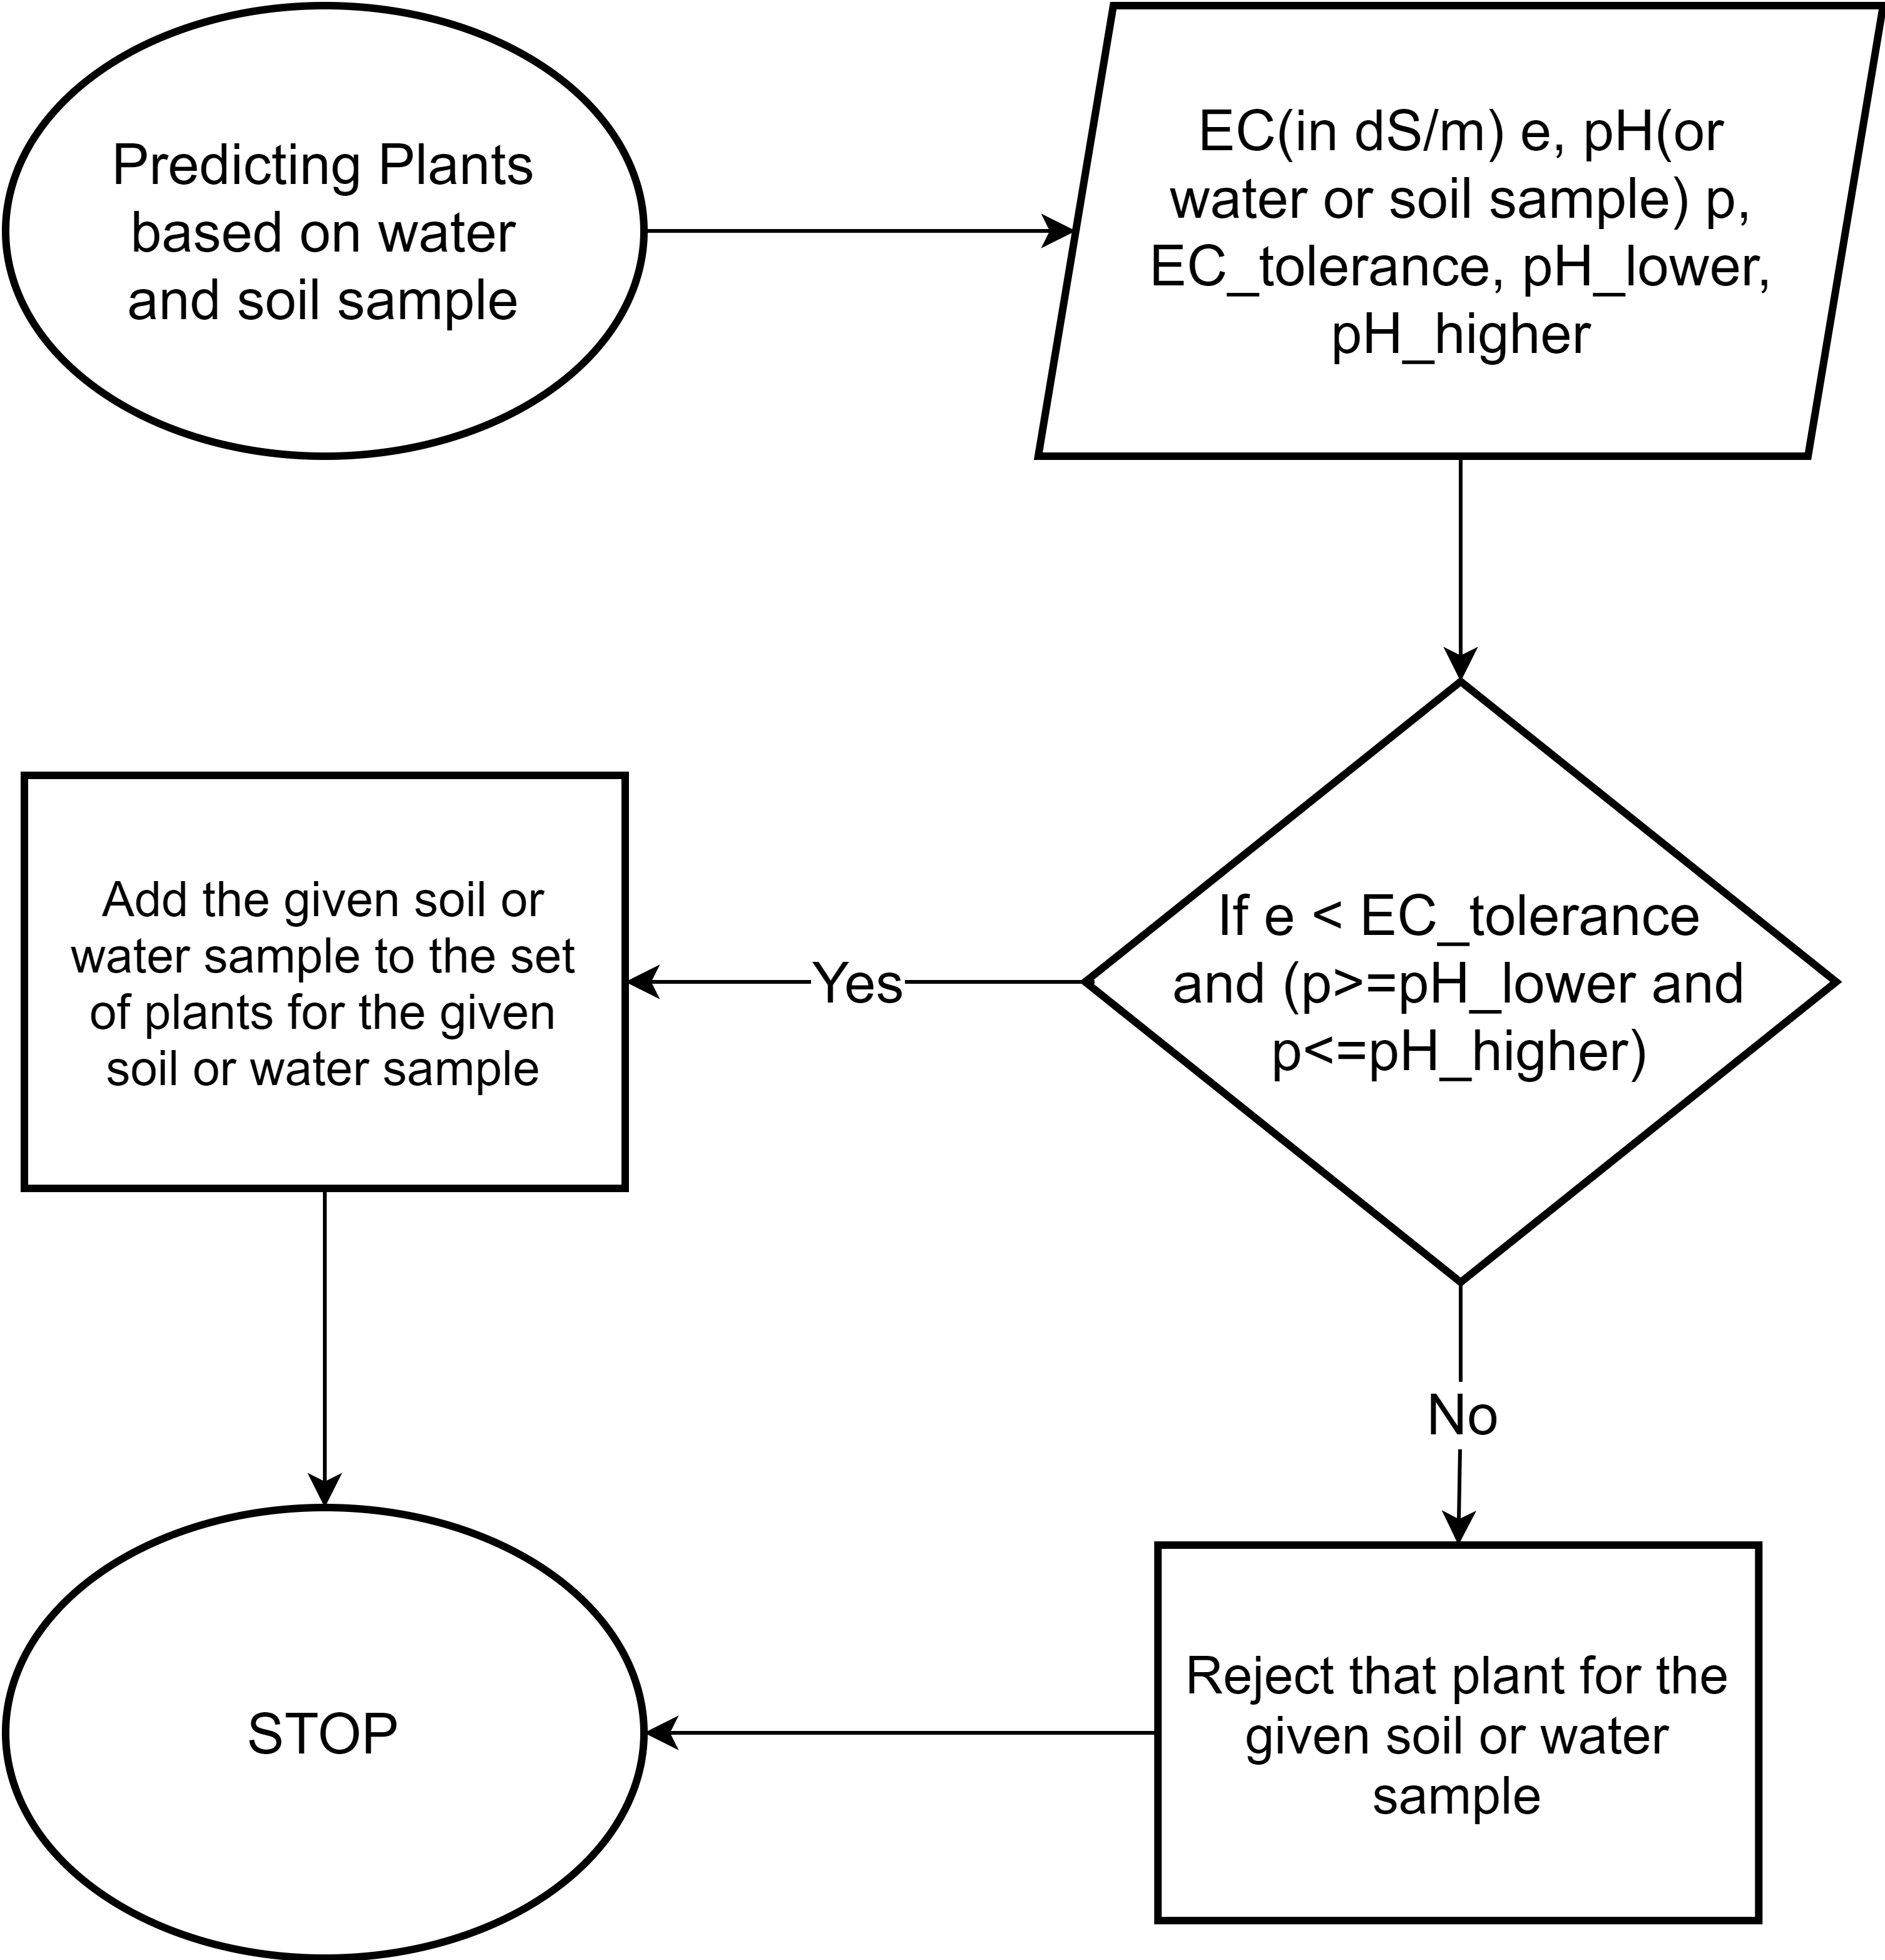
\includegraphics[width=0.7\linewidth]{Model for suggesting plants.png}
\centering
\caption{Calculating IWQI and suggesting the best plants for a given water or soil sample}
\label{fig:phAndECRanges}
\end{figure}

\section{Experiments and Results}
\label{section:expAndRes}
The algorithm was implemented in python 3 with pandas and numpy for loading and preprocessing datasets. All of the classification methods were applied using Scikit-learn\cite{article:scikit-learn}. The parameter settings for various classification algorithms are described below in \ref{subsection:parameterSettings}. The evaluation criteria is explained in \ref{subsection:evaluationMetrics} and results in \ref{subsection:resultsOfClassificationBasedOnIWQI} and \ref{subsection:finalResults}. 

\subsection{Parameter Settings for Classification Model}
\label{subsection:parameterSettings}
The parameter settings for all the classifiers are mentioned in Table \ref{table:parametersClassifiers}. Various parameters for the classifiers are as follows:

\renewcommand{\labelitemi}{\textbullet}
\begin{itemize}
    \item \textbf{Decision Tree Classifier:}  criterion: The function which is chosen to evaluate split quality, splitter:choosing the method of splitting at each node, min\_samples\_split: The least number of samples that are required to split an internal node.

    \item \textbf{Naive Bayes Classifier:}  alpha: choosing the additive smoothing parameters(either Laplace or Lidstone) , class\_prior: estimated probability of new outcomes for each class, class\_count: during fitting, number of samples found under each class.

    \item \textbf{Gradient Boosting Classifier:} loss: The function whose loss(or cost) we want to reduce . learning rate: this parameter is used to change the contribution of trees in overall classification, N\_estimators: Stages of boosting to perform. Large value gives better performance.

    \item \textbf{Random Forest Classifier:} n\_estimators:The number of trees we need to consider before max voting or average predictions, criterion:The function which is chosen to evaluate split quality(we can choose either ‘gini’ or ‘entropy’), base\_estimator: base template (typically Decision Tree Classifier) which are used to create sub estimators. 

    \item \textbf{Support Vector Classifier:} C: Regularization Parameter, decision\_shape: The shape of decision function to return, tol:Tolerance for stopping criterion

    \item \textbf{Bagging Classifier:} base\_estimator: base estimator selected to fit on random subspaces of the dataset(by default it is DecisionTree Classifier), n\_estimators: the count of base\_estimators.
    
    \item \textbf{MLPClassifier:} hidden\_layer\_sizes:This is an array of size n-2 in which each element represents size of hidden layers where the layer position is the position of the element in the array, activation: function that determines the output of hidden layer(typically tanh or relu), Learning\_rate: This parameter determines the step size of gradient descent.
\end{itemize}

\begin{table}[H]
    \centering
    \begin{tabular}{|l|l|}
    \hline
        \textbf{Classifier} & \textbf{Parameter Settings} \\ \hline
        Bagging Classifier & base\_estimator:SVC, n\_estimators:10 \\ \hline
        DecisionTree & criterion: gini, splitter: best, min\_samples\_split: 2 \\ \hline
        Naive Bayes & alpha: 1.0, class\_prior: None, class\_count: [ 7059. 15826.  5057.  2055.   402.] \\ \hline
        Gradient Boosting & loss: deviance, learning rate: 0.1, n\_estimators: 100 \\ \hline
        Random Forest & n\_estimators: 100, criterion: gini, base\_estimator\_: DecisionTreeClassifier \\ \hline
        SVM & C: 1.0, decision\_function\_shape: 'ovr', tol:0.001 \\ \hline
        MLP & hidden\_layer\_sizes:128, activation='relu', learning\_rate=0.001 \\ \hline
    \end{tabular}
    \caption{Parameter Settings for Classifiers}
    \label{table:parametersClassifiers}
\end{table}

\subsection{Evaluation Metrics For Classification Model}
\label{subsection:evaluationMetrics}
Classification algorithms used are evaluated using Accuracy, Precision, Recall and F1 score. We also divided the dataset into five parts for cross validation and measured accuracy on each part. Before we define these metrics we need to define different types of result of class predictions which are True positive, False positive, True negative and False negative. When a model correctly predicts positive class it is True Positive(TPos), correct prediction of Negative class is True Negative(TNeg), wrong prediction of positive class is False Positive(FPos) and wrong prediction of negative class is False Negative(FNeg). For multi-class classification, true-positive prediction means that an observation has been assigned a class to which it belongs and negatives occur when observation is assigned to any other class. The metrics we used are explained below:

\begin{itemize}
    \item \textbf{Accuracy:} Is defined as the total number of current predictions divided by total number of predictions. Its formula is given by Equation \ref{equation:accuracy}.
    \item \textbf{Precision:} Precision evaluates the fraction of correct positives which is given by Equation \ref{equation:precision}. 
    \item \textbf{Recall:} Evaluates the fraction of positives that were identified correctly and is given by Equation \ref{equation:recall}.
    \item \textbf{F1 Score:} Combines both precision and recall and can be used independently as an evaluation method for classification algorithms. It is given by Equation \ref{equation:f1Score}.
    \item \textbf{k-Fold cross validation:} Data is first shuffled and then split into k parts. Each part is taken as a test set in turn while the rest of the k-1 parts are a part of the training set. The model is evaluated using this strategy and we can obtain scores for each of the k parts.
    \item \textbf{Confusion Matrix:} It is a matrix of dimension NXN where N is the number of classes which a classification model predicts. Each row corresponds to the actual prediction for that class and column corresponds to predicted prediction for that class. Each cell in this matrix denotes the number of samples predicted as class X where actual class was Y. This helps us to compute accuracy, precision, recall and F1 score.
\end{itemize}

\begin{equation}
\label{equation:accuracy}
    Accuracy = \frac{TPos + TNeg}{TPos + TNeg + FPos + FNeg}
\end{equation}

\begin{equation}
\label{equation:precision}
    Precision(P) = \frac{TPos}{TPos + FPos}
\end{equation}

\begin{equation}
\label{equation:recall}
    Recall(R) = \frac{TPos}{TPos + FNeg}
\end{equation}

\begin{equation}
\label{equation:f1Score}
    F1 Score = 2*\frac{P*R}{P+R}
\end{equation}

\subsection{Results of Classification based on IWQI}
\label{subsection:resultsOfClassificationBasedOnIWQI}
We applied Algorithm 1 on the major ions dataset with 70-30 train-test split and evaluated it with the metrics defined in 5.2. The confusion matrix for all the classification algorithms are shown in Fig. \ref{fig:confusionMatrixForAllAlgos}. For this experiment, we have assigned the numbers to IWQI range with 0-40 as 0, 40-55 as 1, 55-70 as 2, 70-85 as 3 and 85-100 as 4. For the major ions dataset, there are the least number of samples belonging to class 4(495 out of 37999) which is not enough size for classification and hence the poor performance of all the algorithms for that class. For all other classes 0-3, the algorithm performs well except for Naive Bayes Classifier. Using the confusion matrix from Fig. \ref{fig:confusionMatrixForAllAlgos} and Equations \ref{equation:accuracy},\ref{equation:precision},\ref{equation:recall} and \ref{equation:f1Score}, we calculated the Precision, Recall, Accuracy and F1 Score in Table \ref{table:classificationResults}. Random forest has the best performance with accuracy of 86.9\% followed by Gradient Boosting(85.8\%) and MLP classifier(84.6\%). Performance of Naive Bayes is the worst with an accuracy of 52.6\% and F1 Score of 13.8\%. We also performed 5-fold validation for our methods whose results are given in Table \ref{table:fiveFoldCrossValidation} where Random Forest performs the best and Naive Bayes performs the worst.

\begin{table}[H]
    \centering
    \begin{tabular}{|l|l|l|l|l|}
    \hline
        \textbf{Methods} & \textbf{Accuracy} & \textbf{Precision} & \textbf{Recall} & \textbf{F1} \\ \hline
        DecisionTree & 0.832 & 0.728 & 0.740 & 0.733 \\ \hline
        Naive Bayes & 0.526 & 0.105 & 0.200 & 0.138 \\ \hline
        Gradient Boosting & 0.858 & 0.762 & 0.757 & 0.760 \\ \hline
        Random Forest & \textbf{0.869} & \textbf{0.790} & \textbf{0.765} & \textbf{0.776} \\ \hline
        SVM & 0.845 & 0.762 & 0.711 & 0.726 \\ \hline
        Bagging & 0.813 & 0.750 & 0.664 & 0.690 \\ \hline
        MLP & 0.846 & 0.734 & 0.743 & 0.738 \\ \hline
    \end{tabular}
    \caption{Classification results for algorithm 1}
    \label{table:classificationResults}
\end{table}

\begin{table}[H]
    \centering
    \begin{tabular}{|l|l|l|l|l|l|}
    \hline
        \textbf{Five Fold Cross Validation} &  &  &  &  &  \\ \hline
        \textbf{Methods} & \textbf{Fold 1} & \textbf{Fold 2} & \textbf{Fold 3} & \textbf{Fold 4} & \textbf{Fold 5} \\ \hline
        Bagging Classifier & 0.829 & 0.823 & 0.814 & 0.830 & 0.813 \\ \hline
        DecisionTree & 0.833 & 0.836 & 0.828 & 0.823 & 0.839 \\ \hline
        Naive Bayes & 0.518 & 0.518 & 0.518 & 0.518 & 0.519 \\ \hline
        Gradient Boosting & 0.862 & 0.866 & 0.869 & 0.859 & 0.862 \\ \hline
        Random Forest & \textbf{0.866} & \textbf{0.870} & \textbf{0.870} & \textbf{0.862} & \textbf{0.871} \\ \hline
        SVM & 0.853 & 0.849 & 0.846 & 0.841 & 0.848 \\ \hline
        MLP & 0.847 & 0.853 & 0.857 & 0.847 & 0.849 \\ \hline
    \end{tabular}
    \caption{Five fold cross validation scores for algorithm 1}
    \label{table:fiveFoldCrossValidation}
\end{table}


\begin{figure}[H]
\centering

\begin{subfigure}{.49\textwidth}
  \centering
  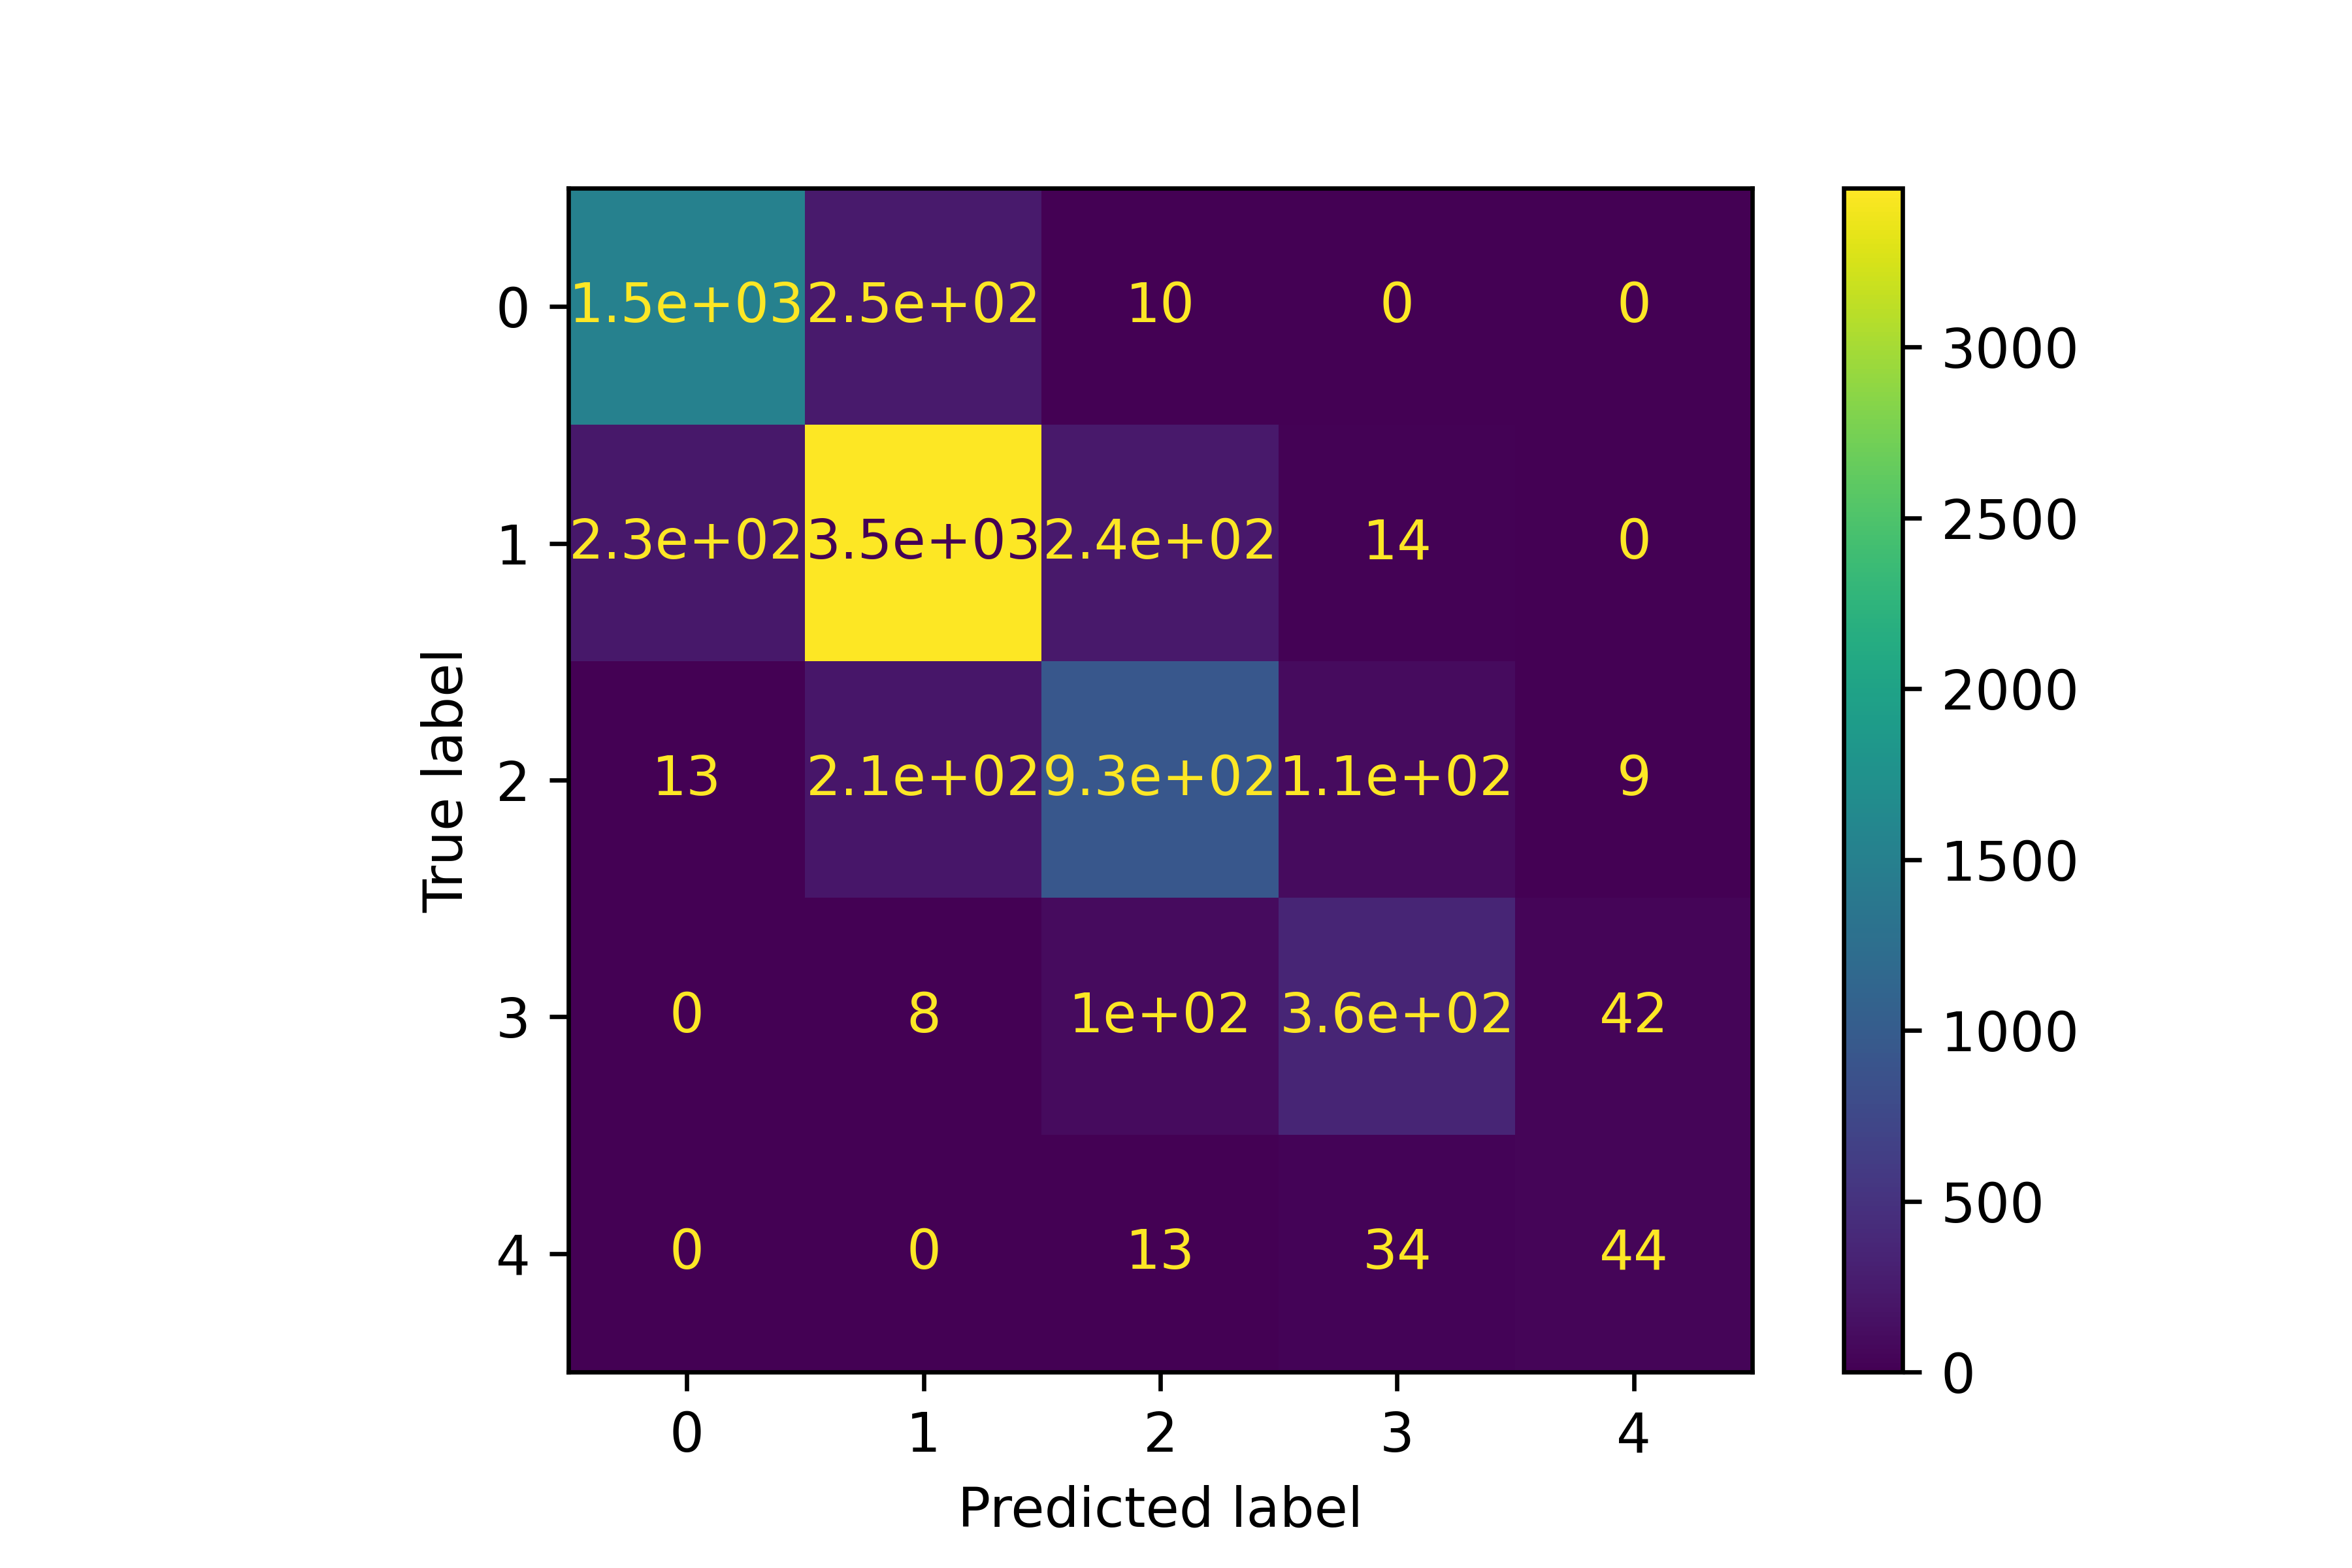
\includegraphics[width=\linewidth]{decisionTreeConfusionMatrix.png} 
  \caption{}
%   \caption{Confusion Matrix for Decision Tree}
  \label{subfig:decisionTree}
\end{subfigure}
\begin{subfigure}{.49\textwidth}
  \centering
  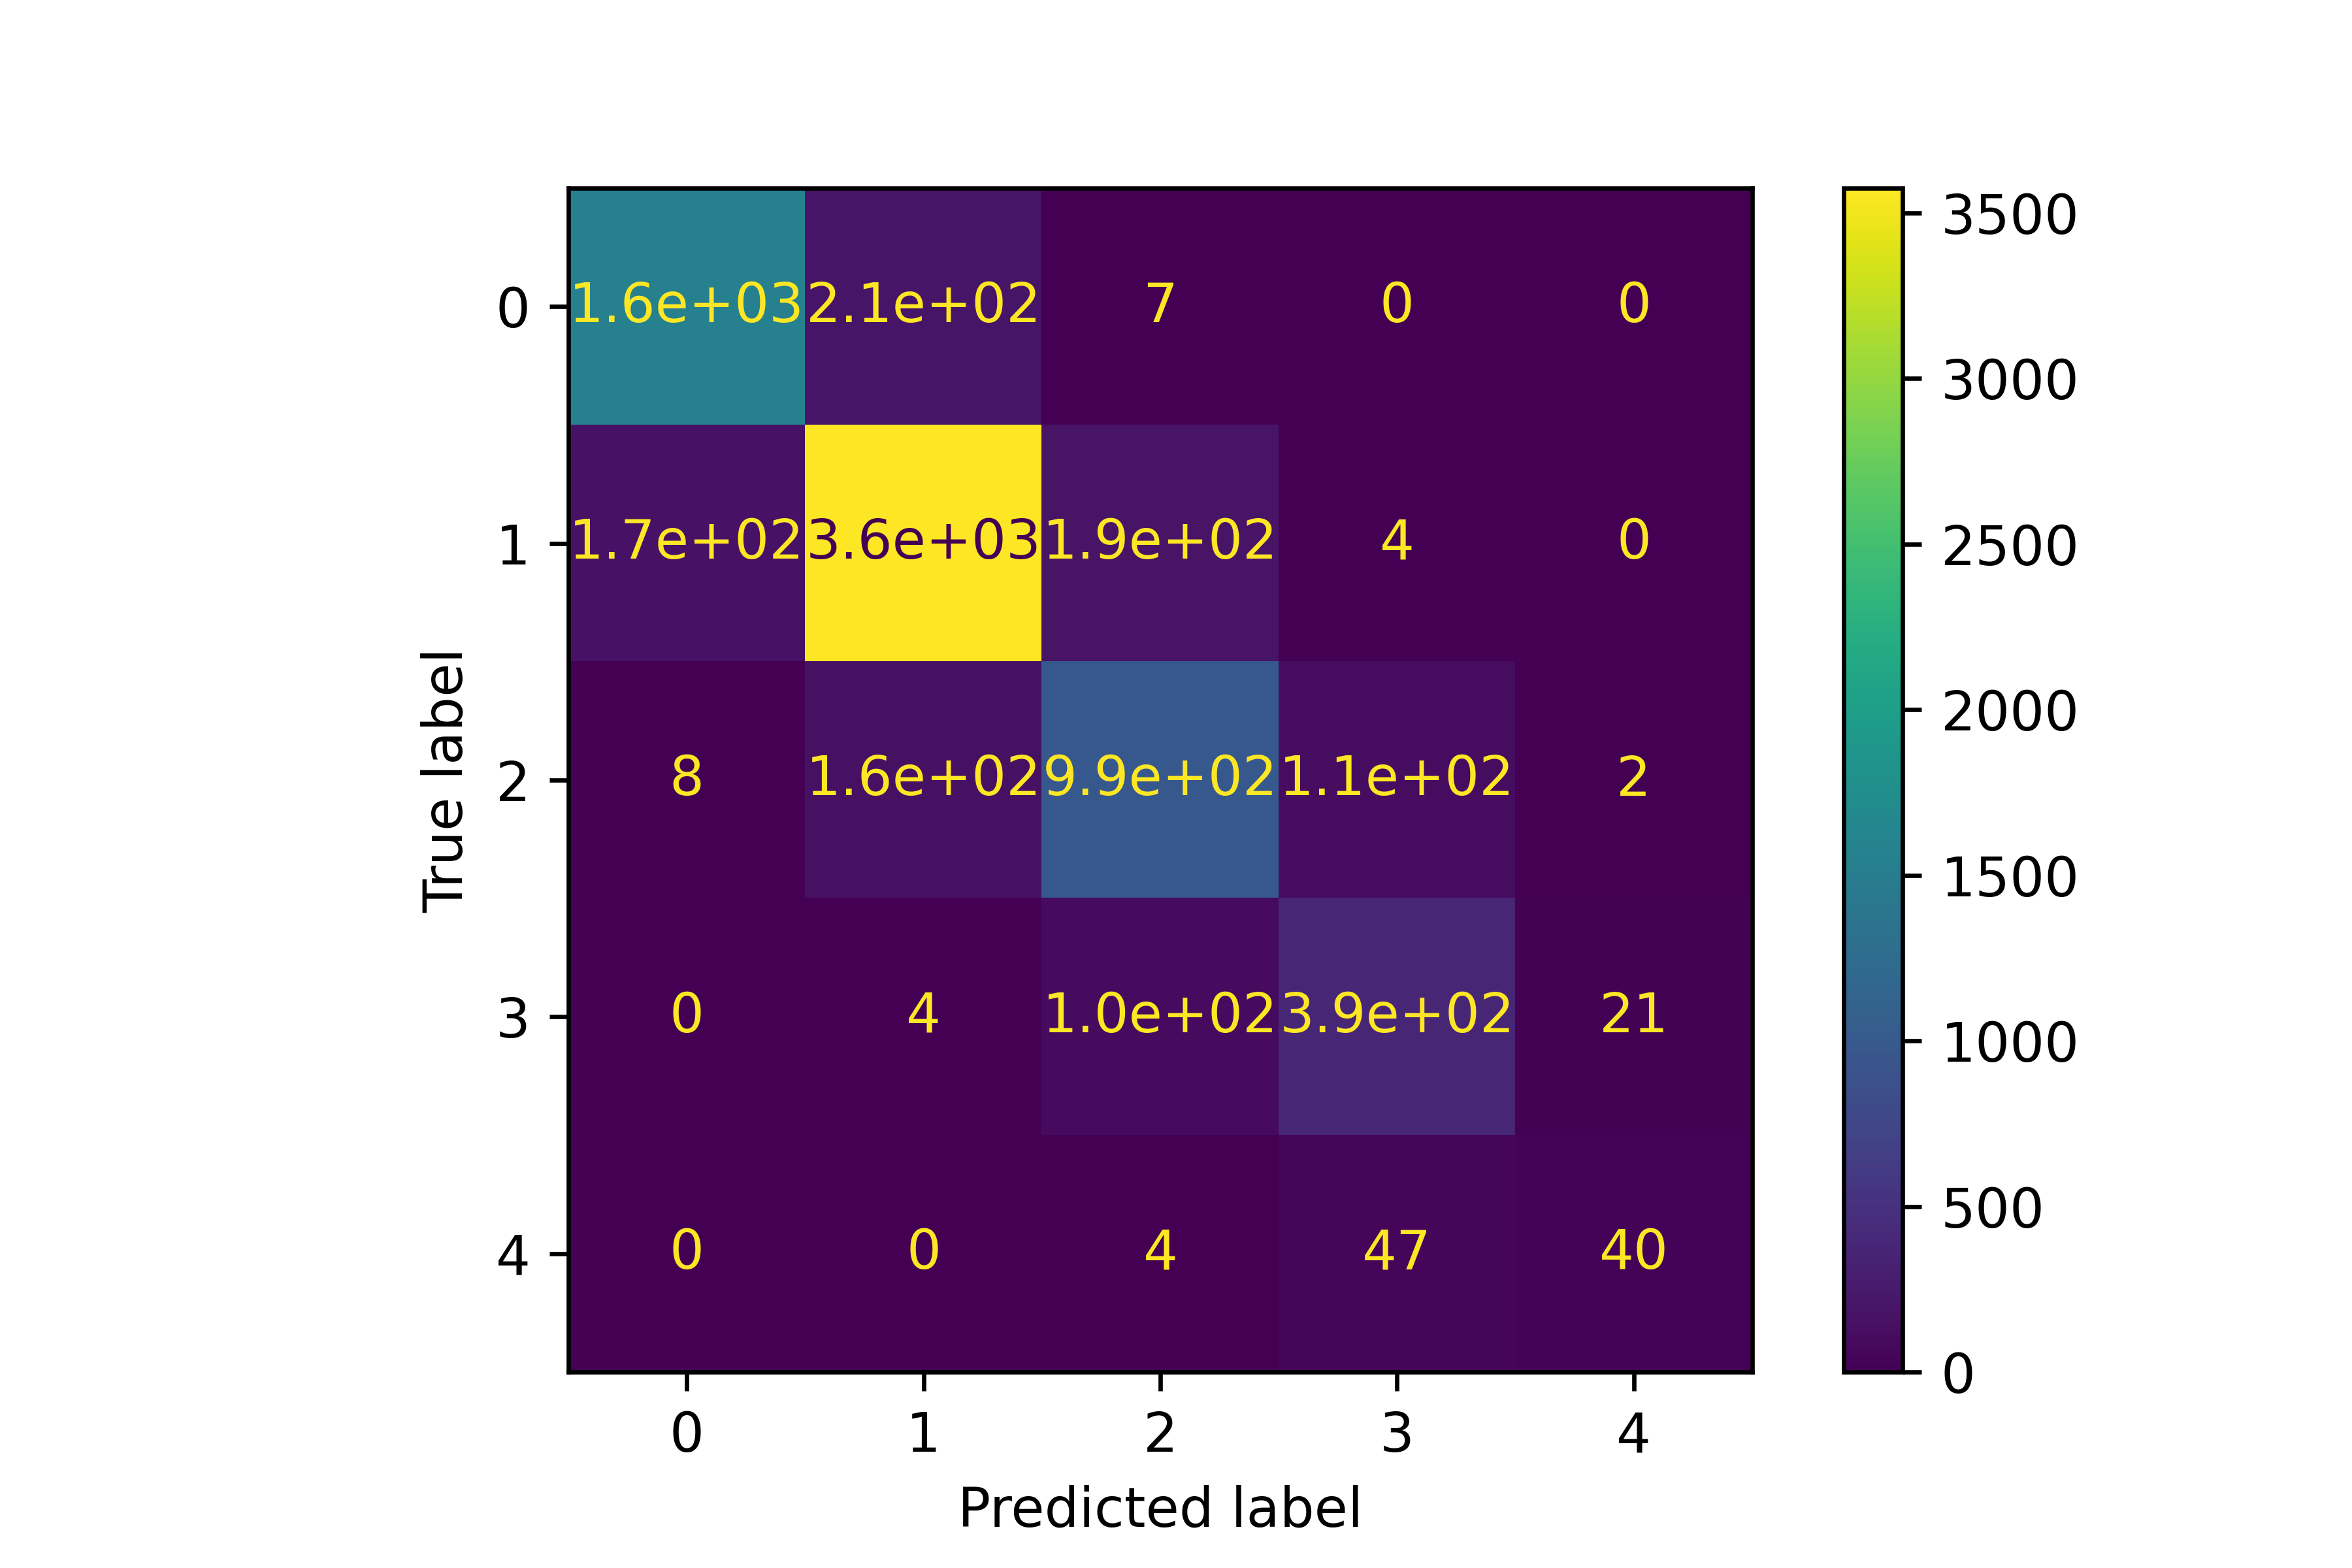
\includegraphics[width=\linewidth]{gradientBoostConfusionMatrix.png}  
  \caption{}
%   \caption{Confusion Matrix for Gradient Boost}
  \label{subfig:gradientBoost}
\end{subfigure}

\begin{subfigure}{.49\textwidth}
  \centering
  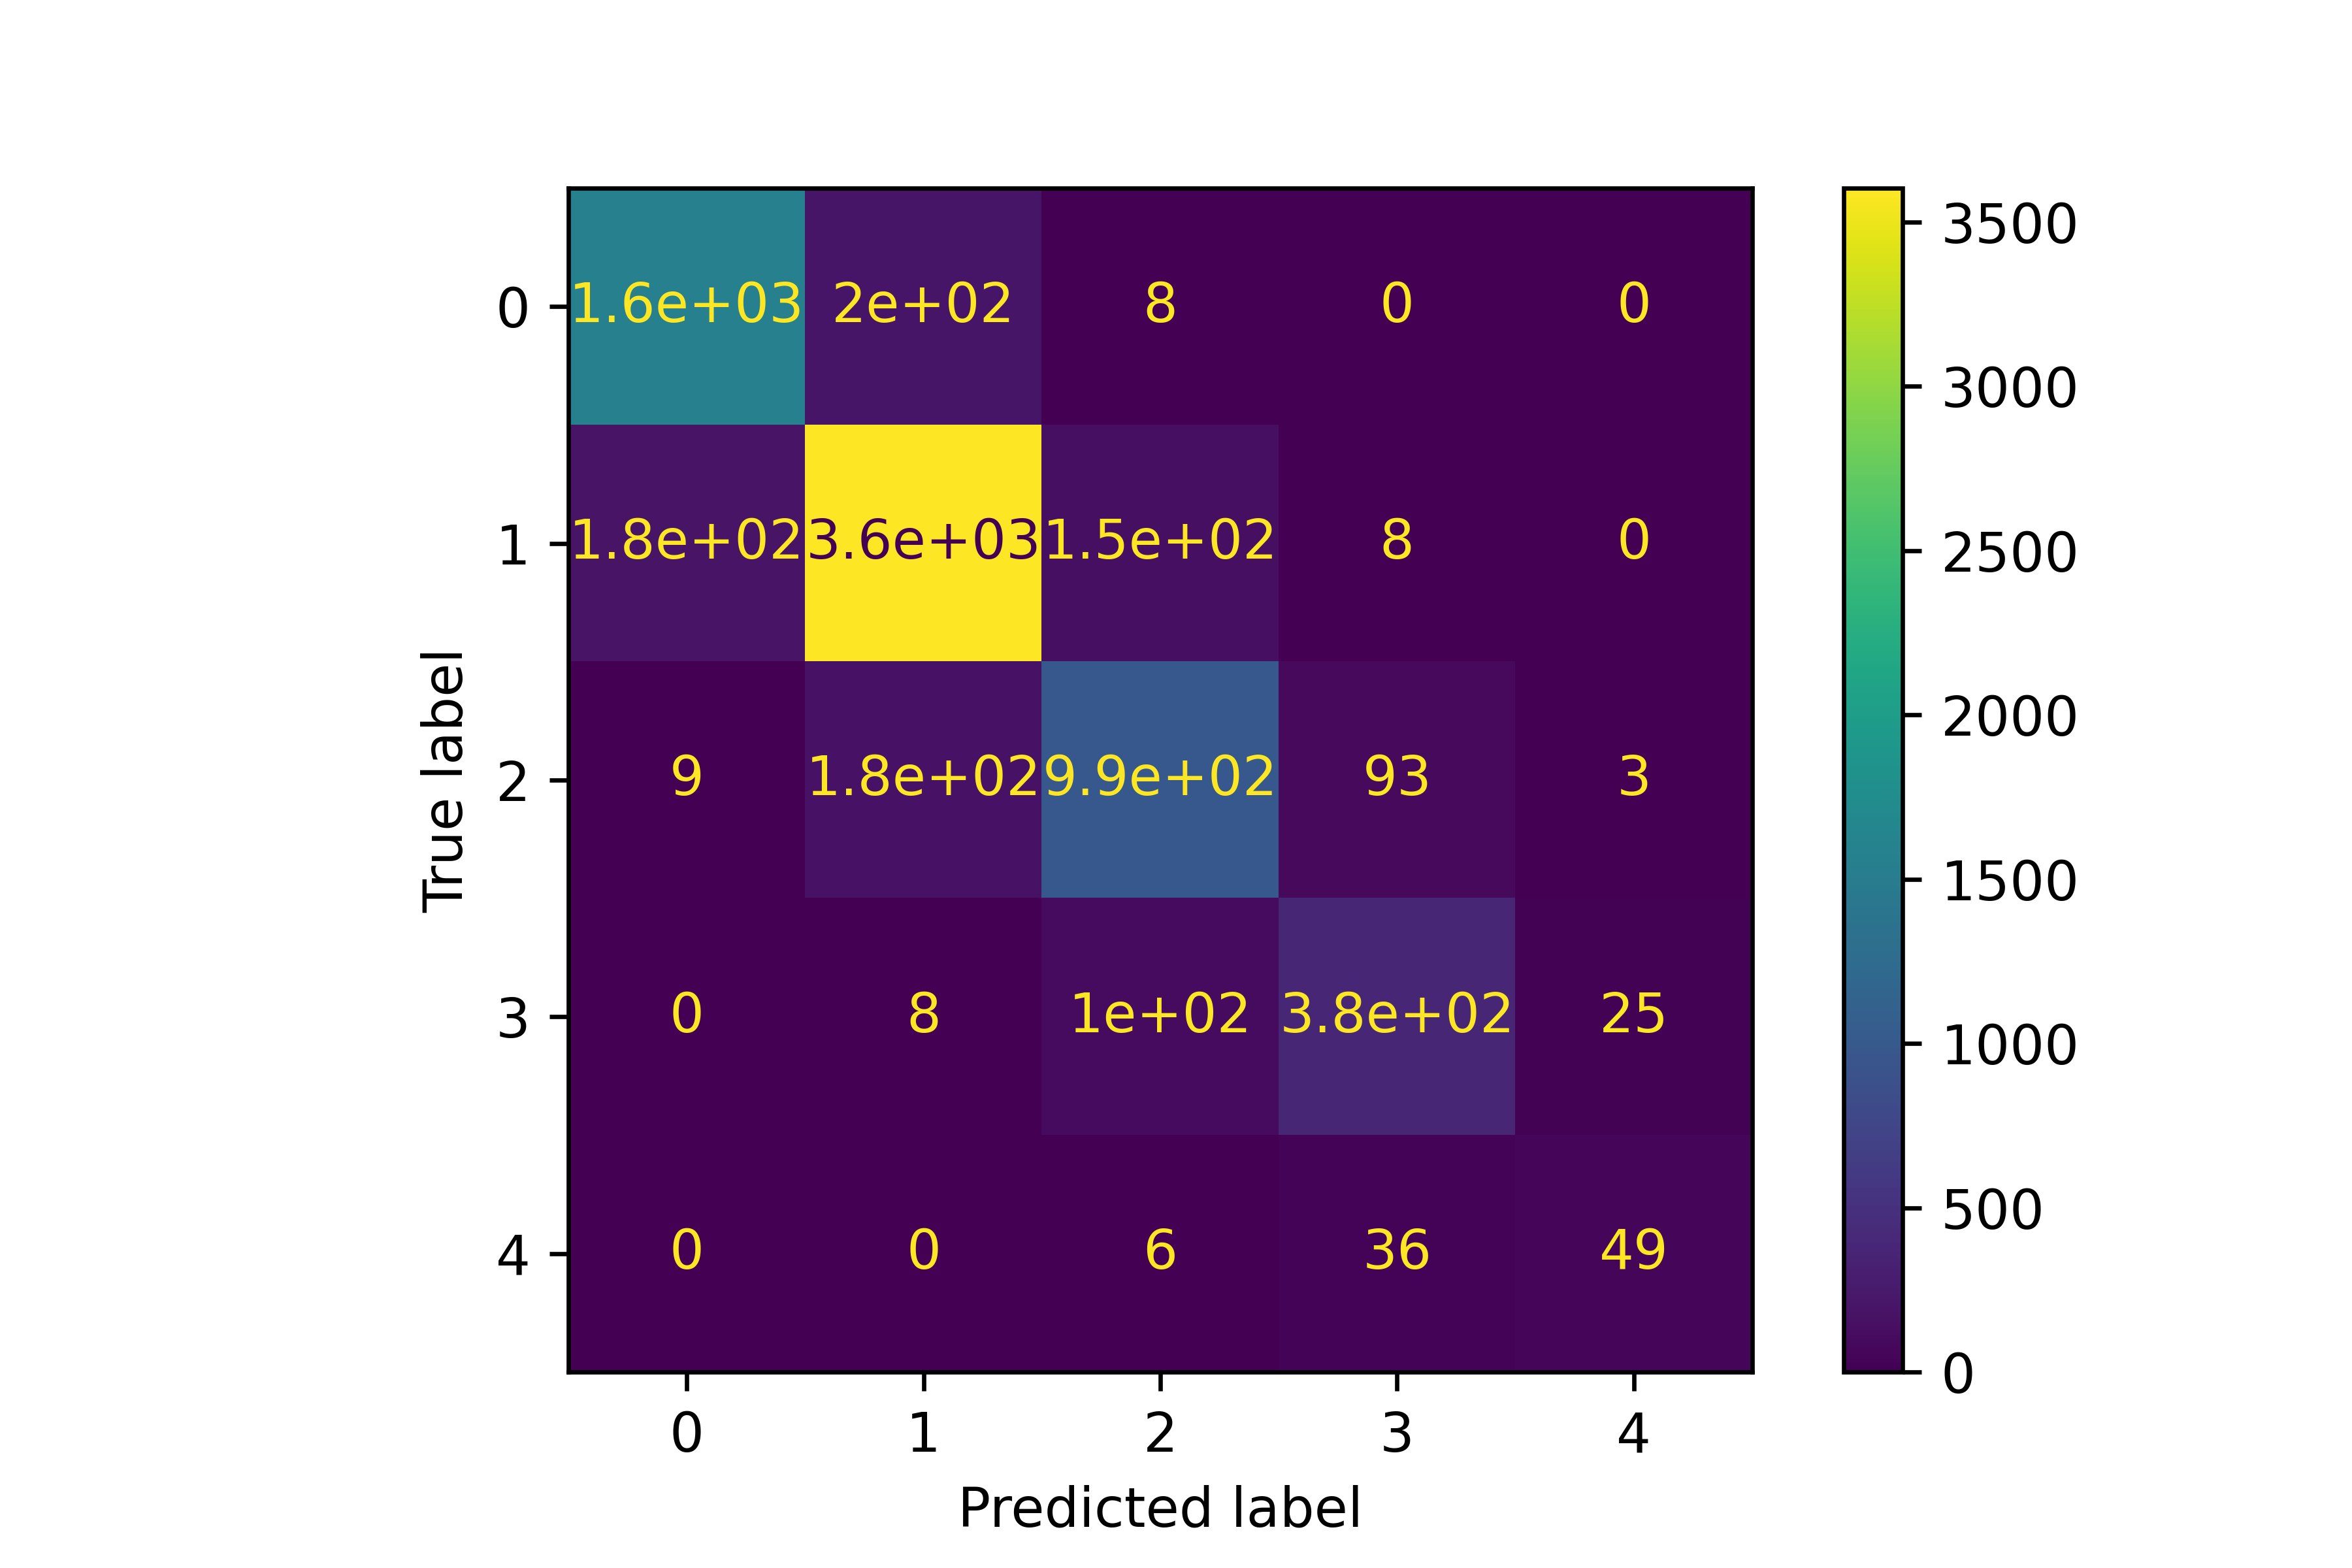
\includegraphics[width=\linewidth]{randomForestConfusionMatrix.png}  
  \caption{}
%   \caption{Confusion Matrix for Random Forest}
  \label{subfig:randomForest}
\end{subfigure}
\begin{subfigure}{.49\textwidth}
  \centering
  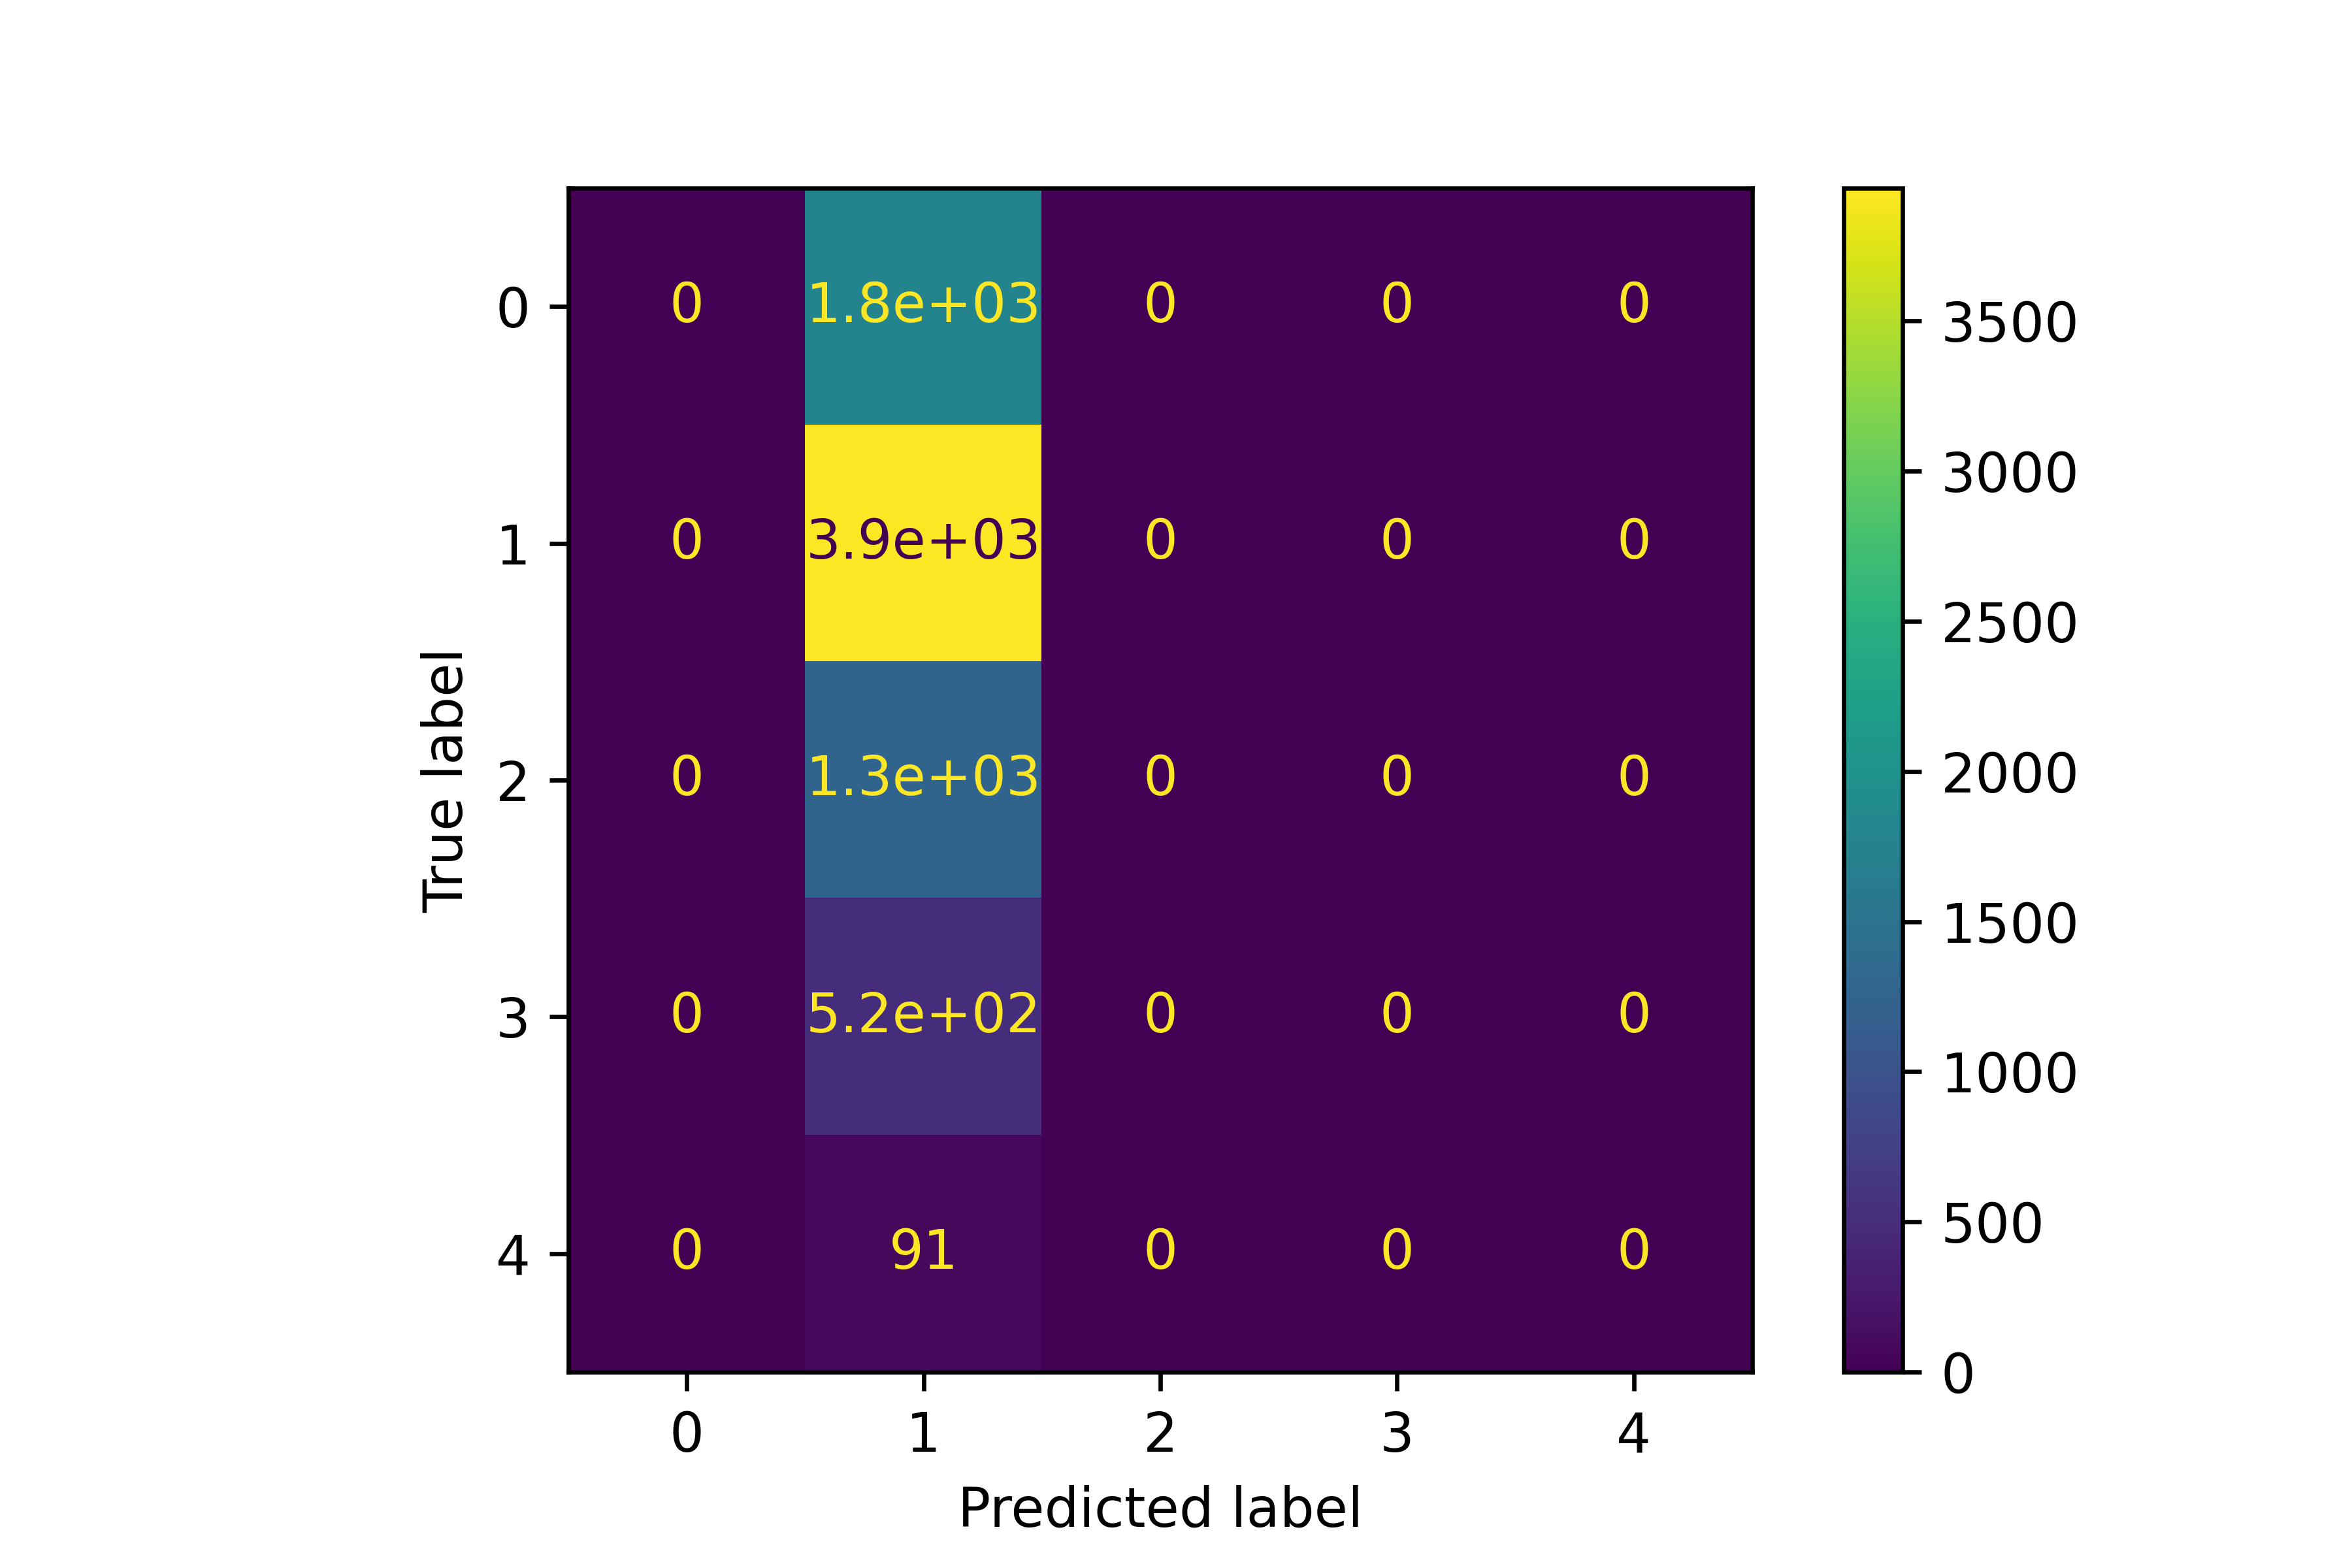
\includegraphics[width=\linewidth]{multinomialNaiveBayesConfusionMatrix.png} 
  \caption{}
%   \caption{Confusion Matrix for Naive Bayes}
  \label{subfig:naiveBayes}
\end{subfigure}

\begin{subfigure}{.49\textwidth}
  \centering
  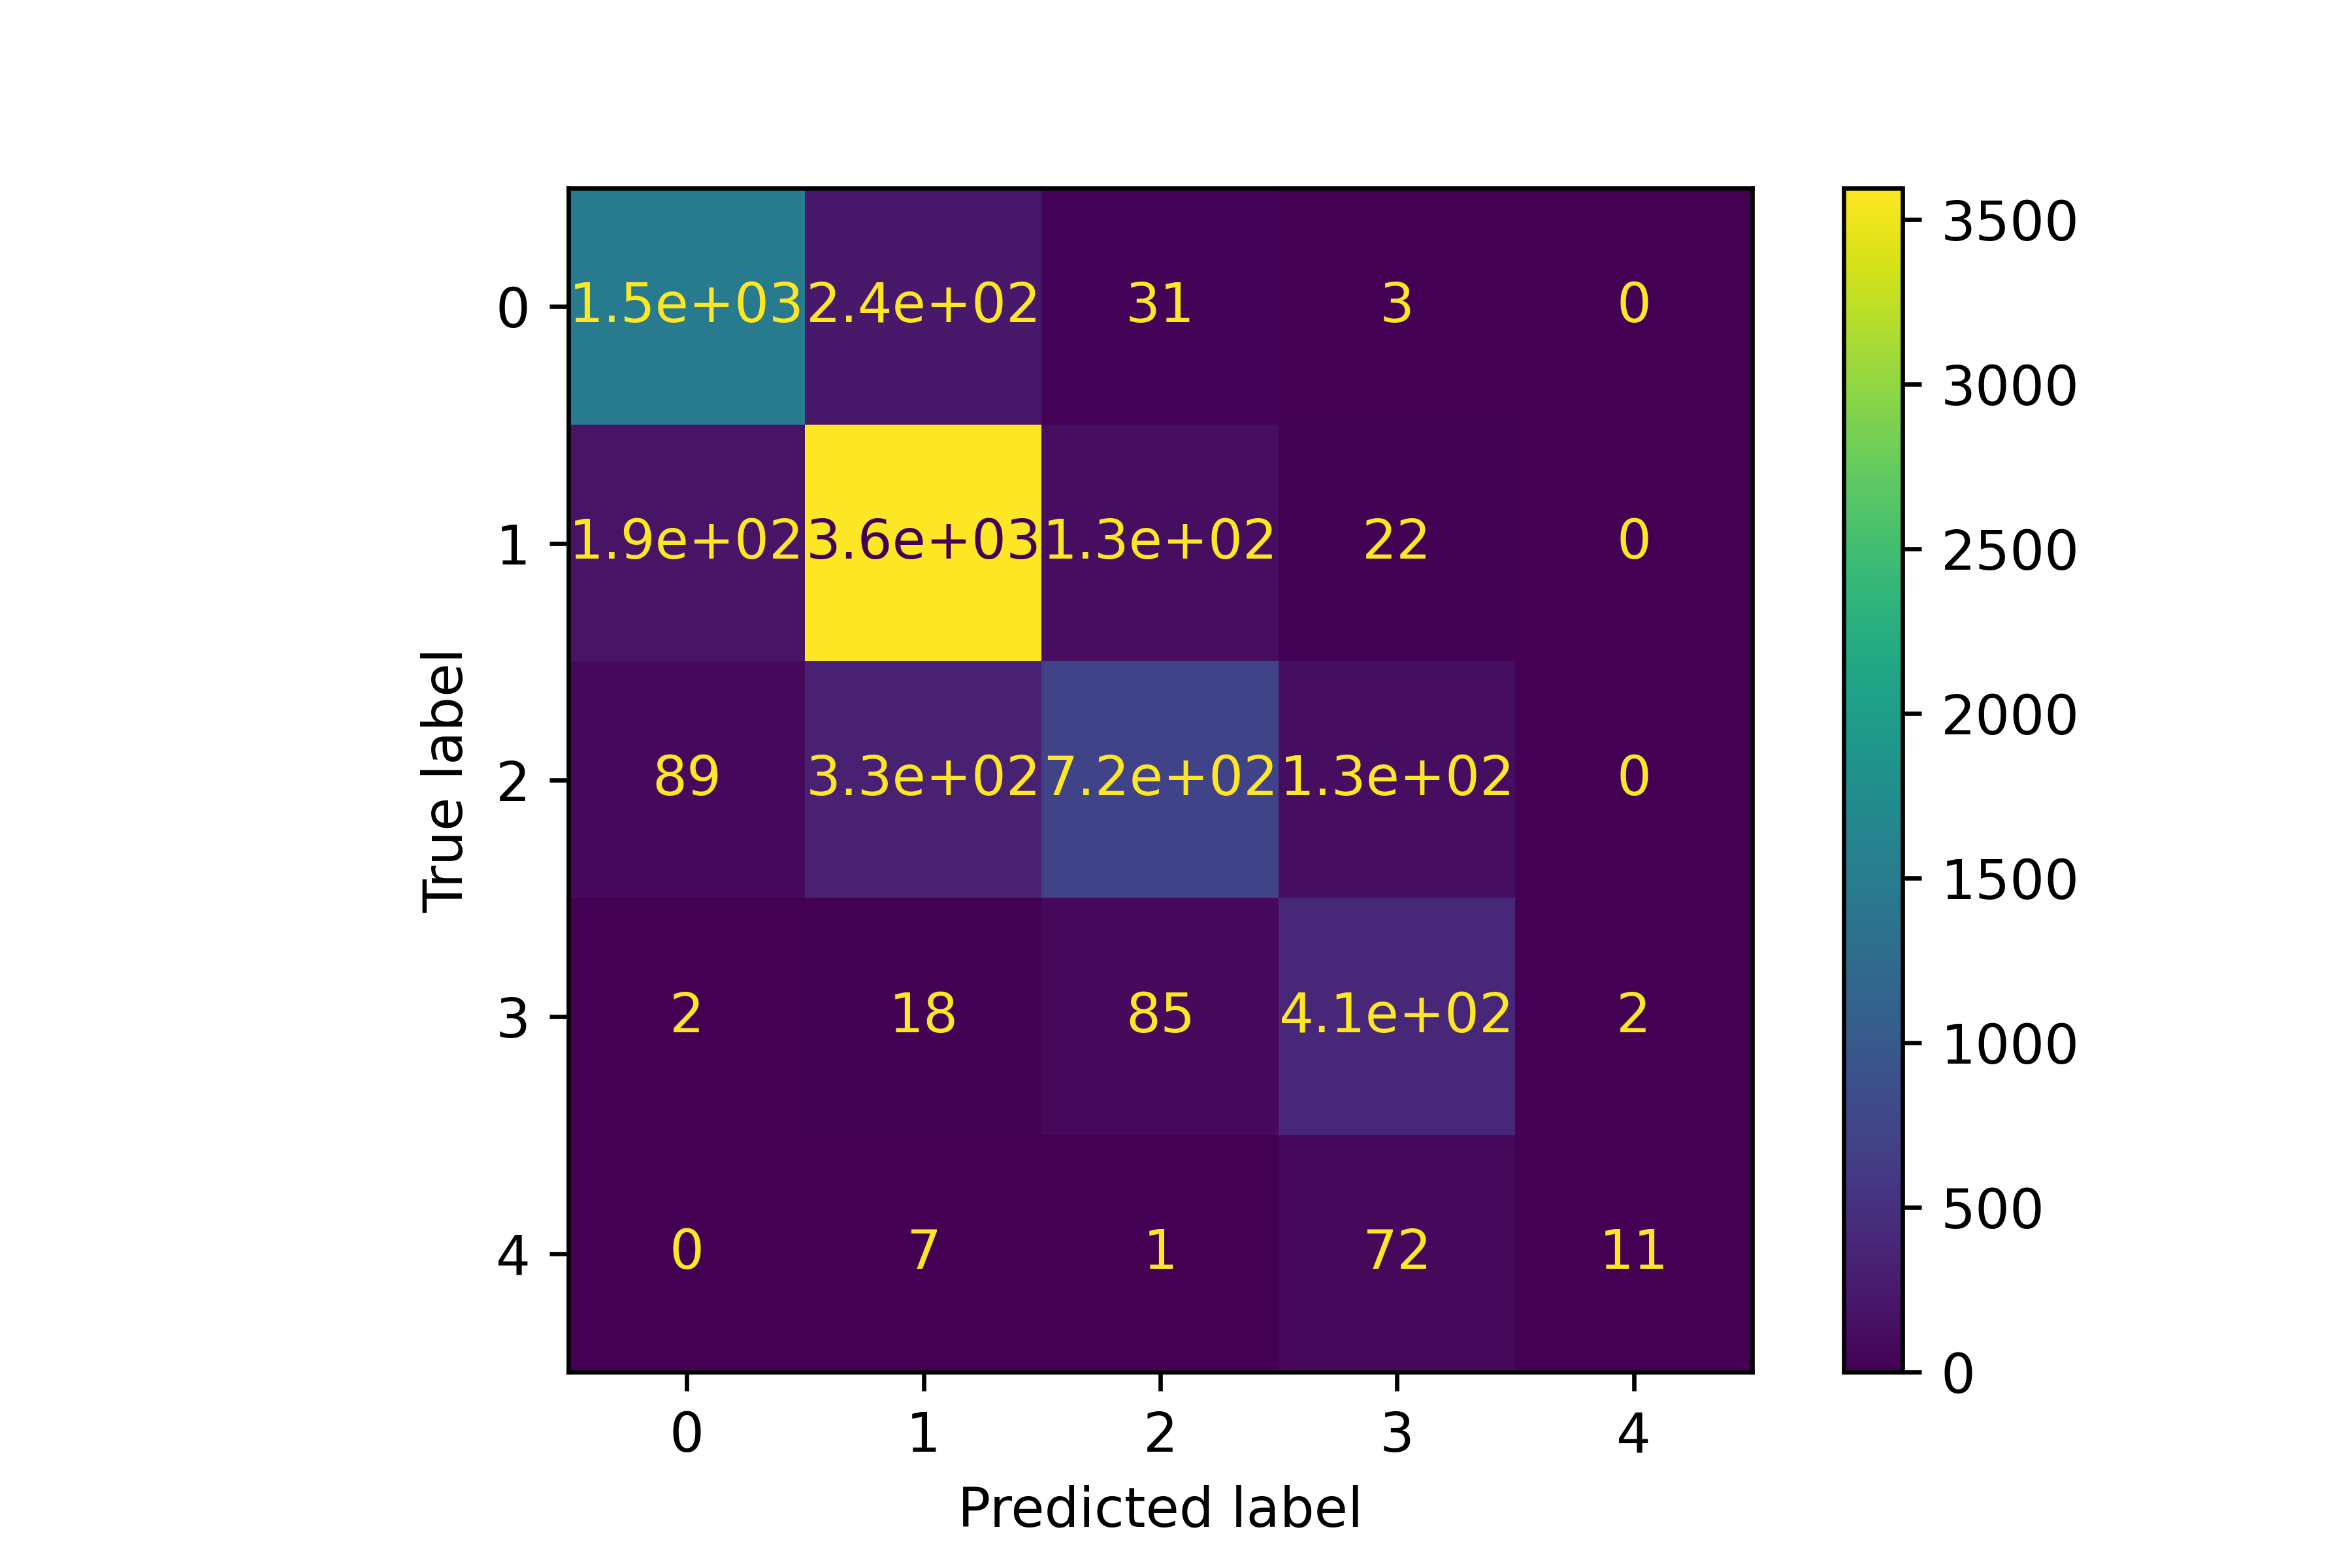
\includegraphics[width=\linewidth]{baggingConfusionMatrix.png} 
  \caption{}
%   \caption{Confusion Matrix for Bagging Classifer}
  \label{subfig:bagging}
\end{subfigure}
\begin{subfigure}{.49\textwidth}
  \centering
  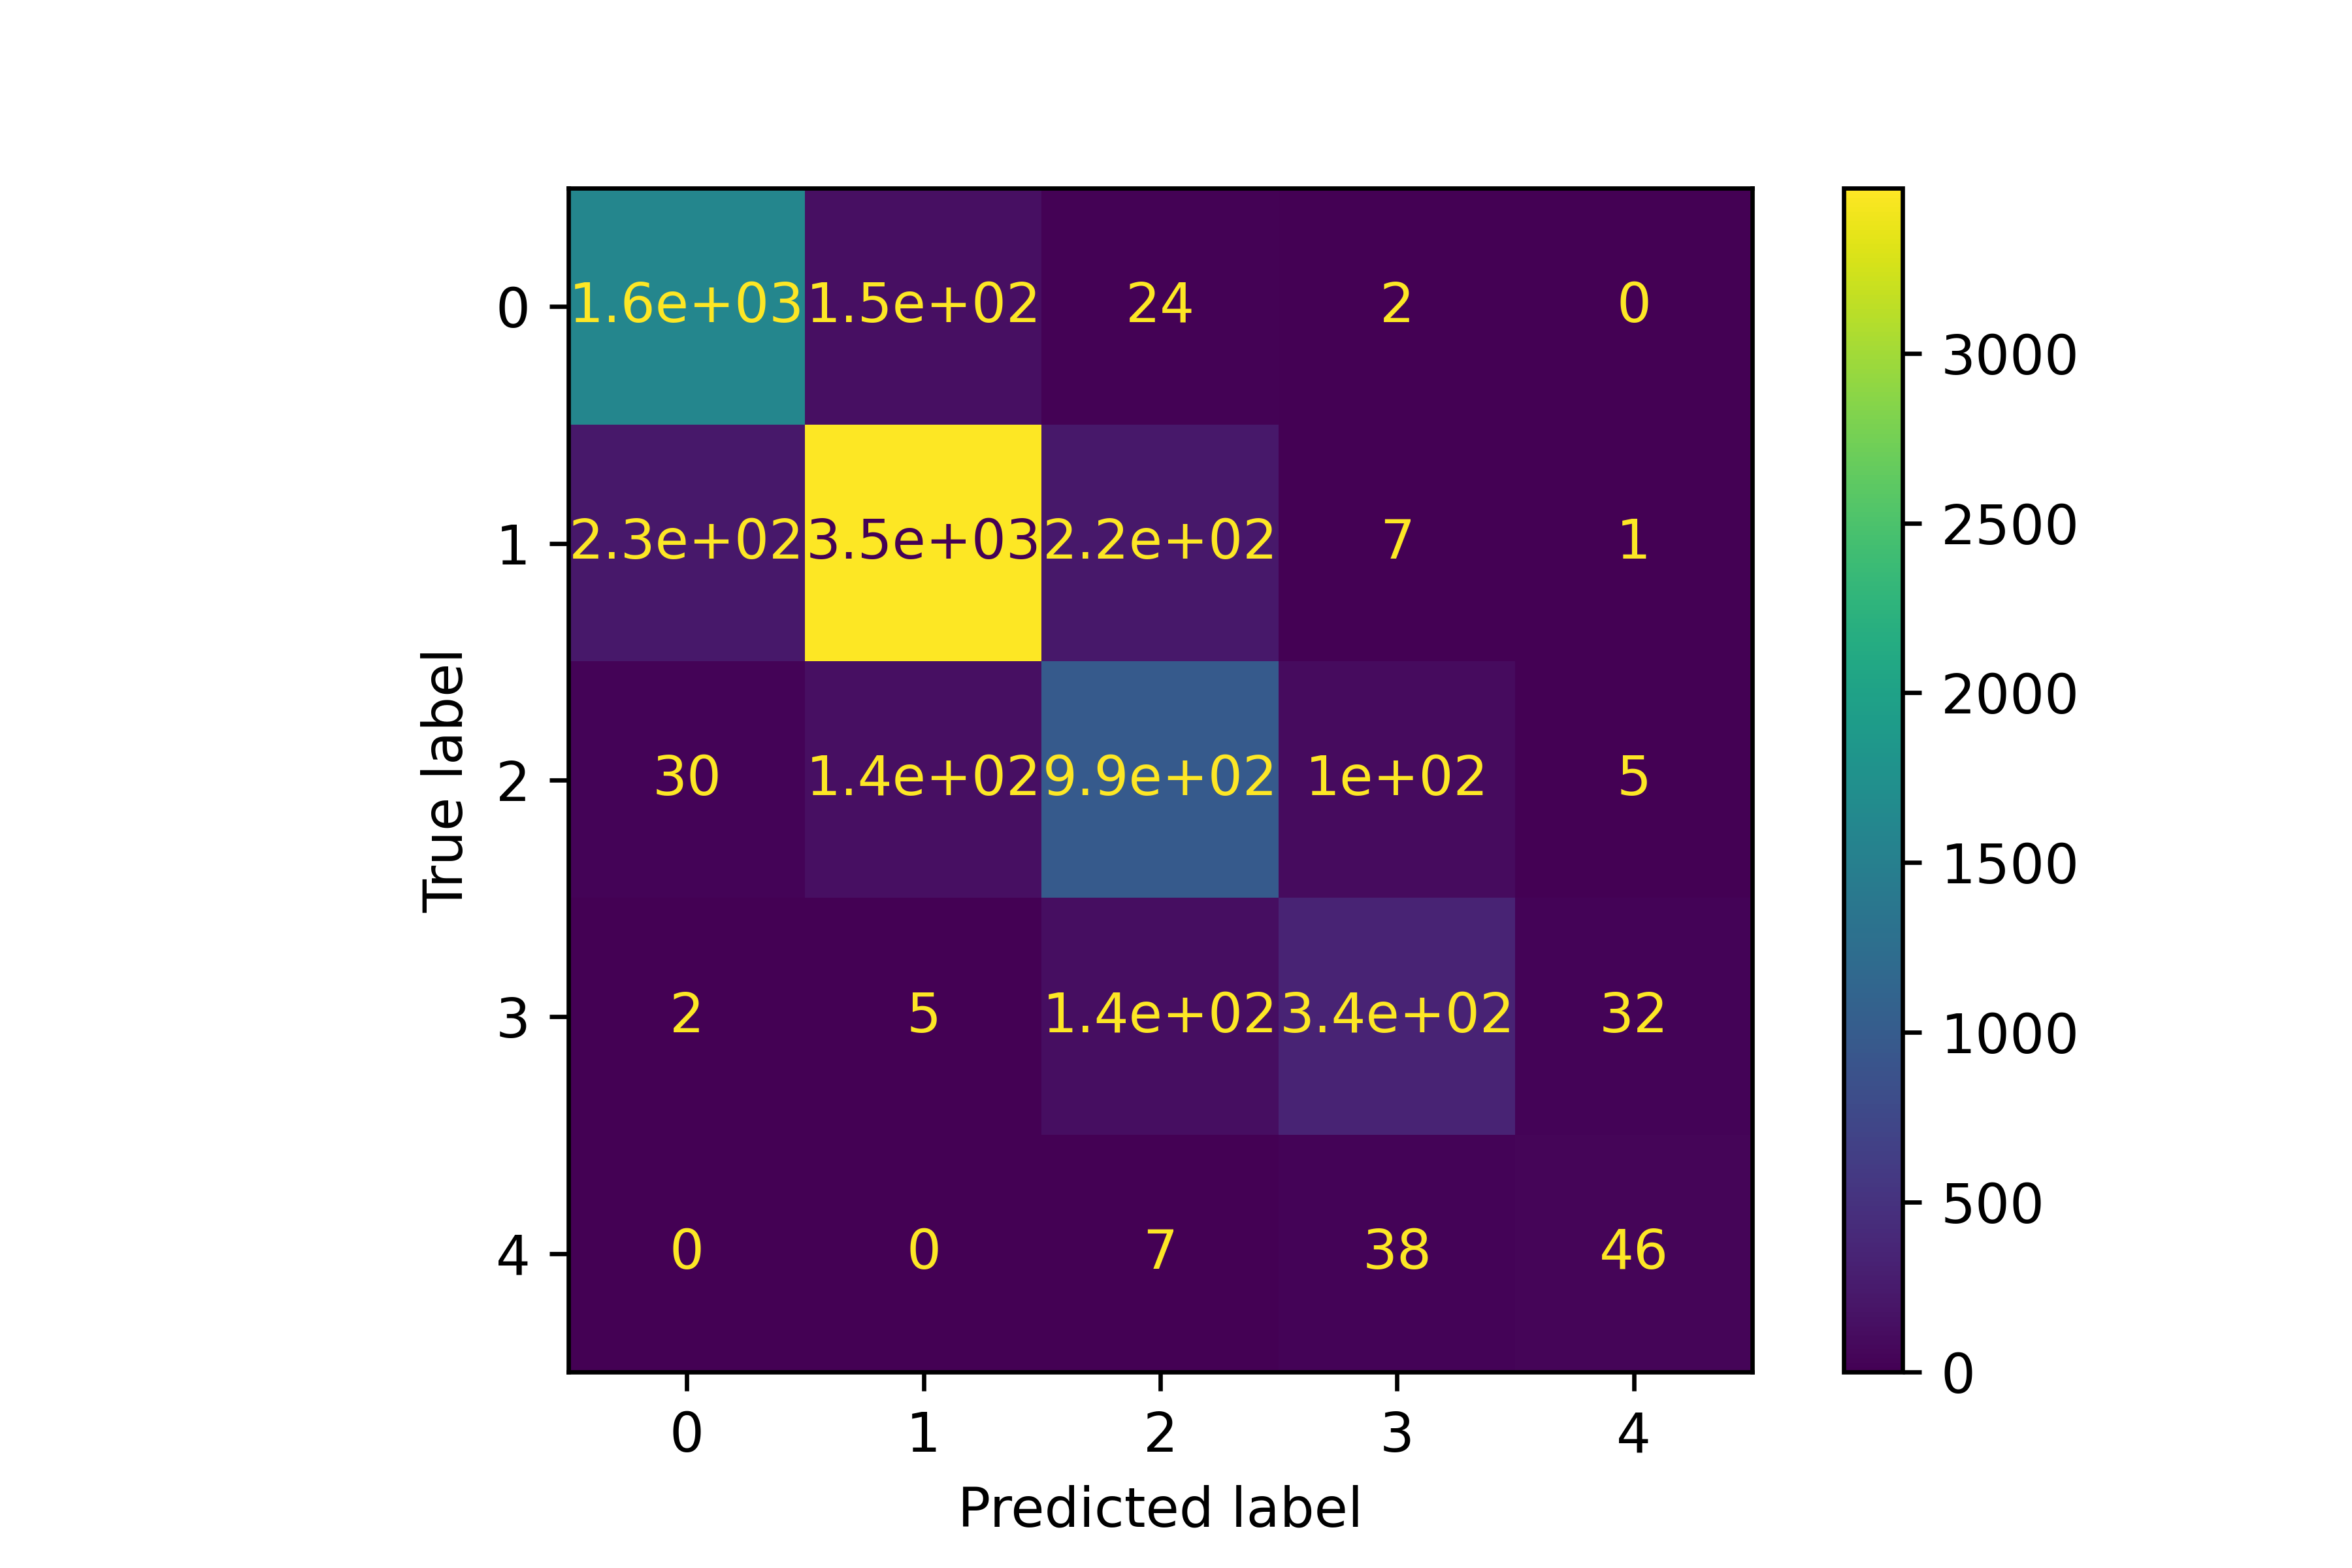
\includegraphics[width=\linewidth]{mlpConfusionMatrix.png}  
  \caption{}
%   \caption{Confusion Matrix for ANN}
  \label{subfig:ann}
\end{subfigure}

\begin{subfigure}{.49\textwidth}
  \centering
  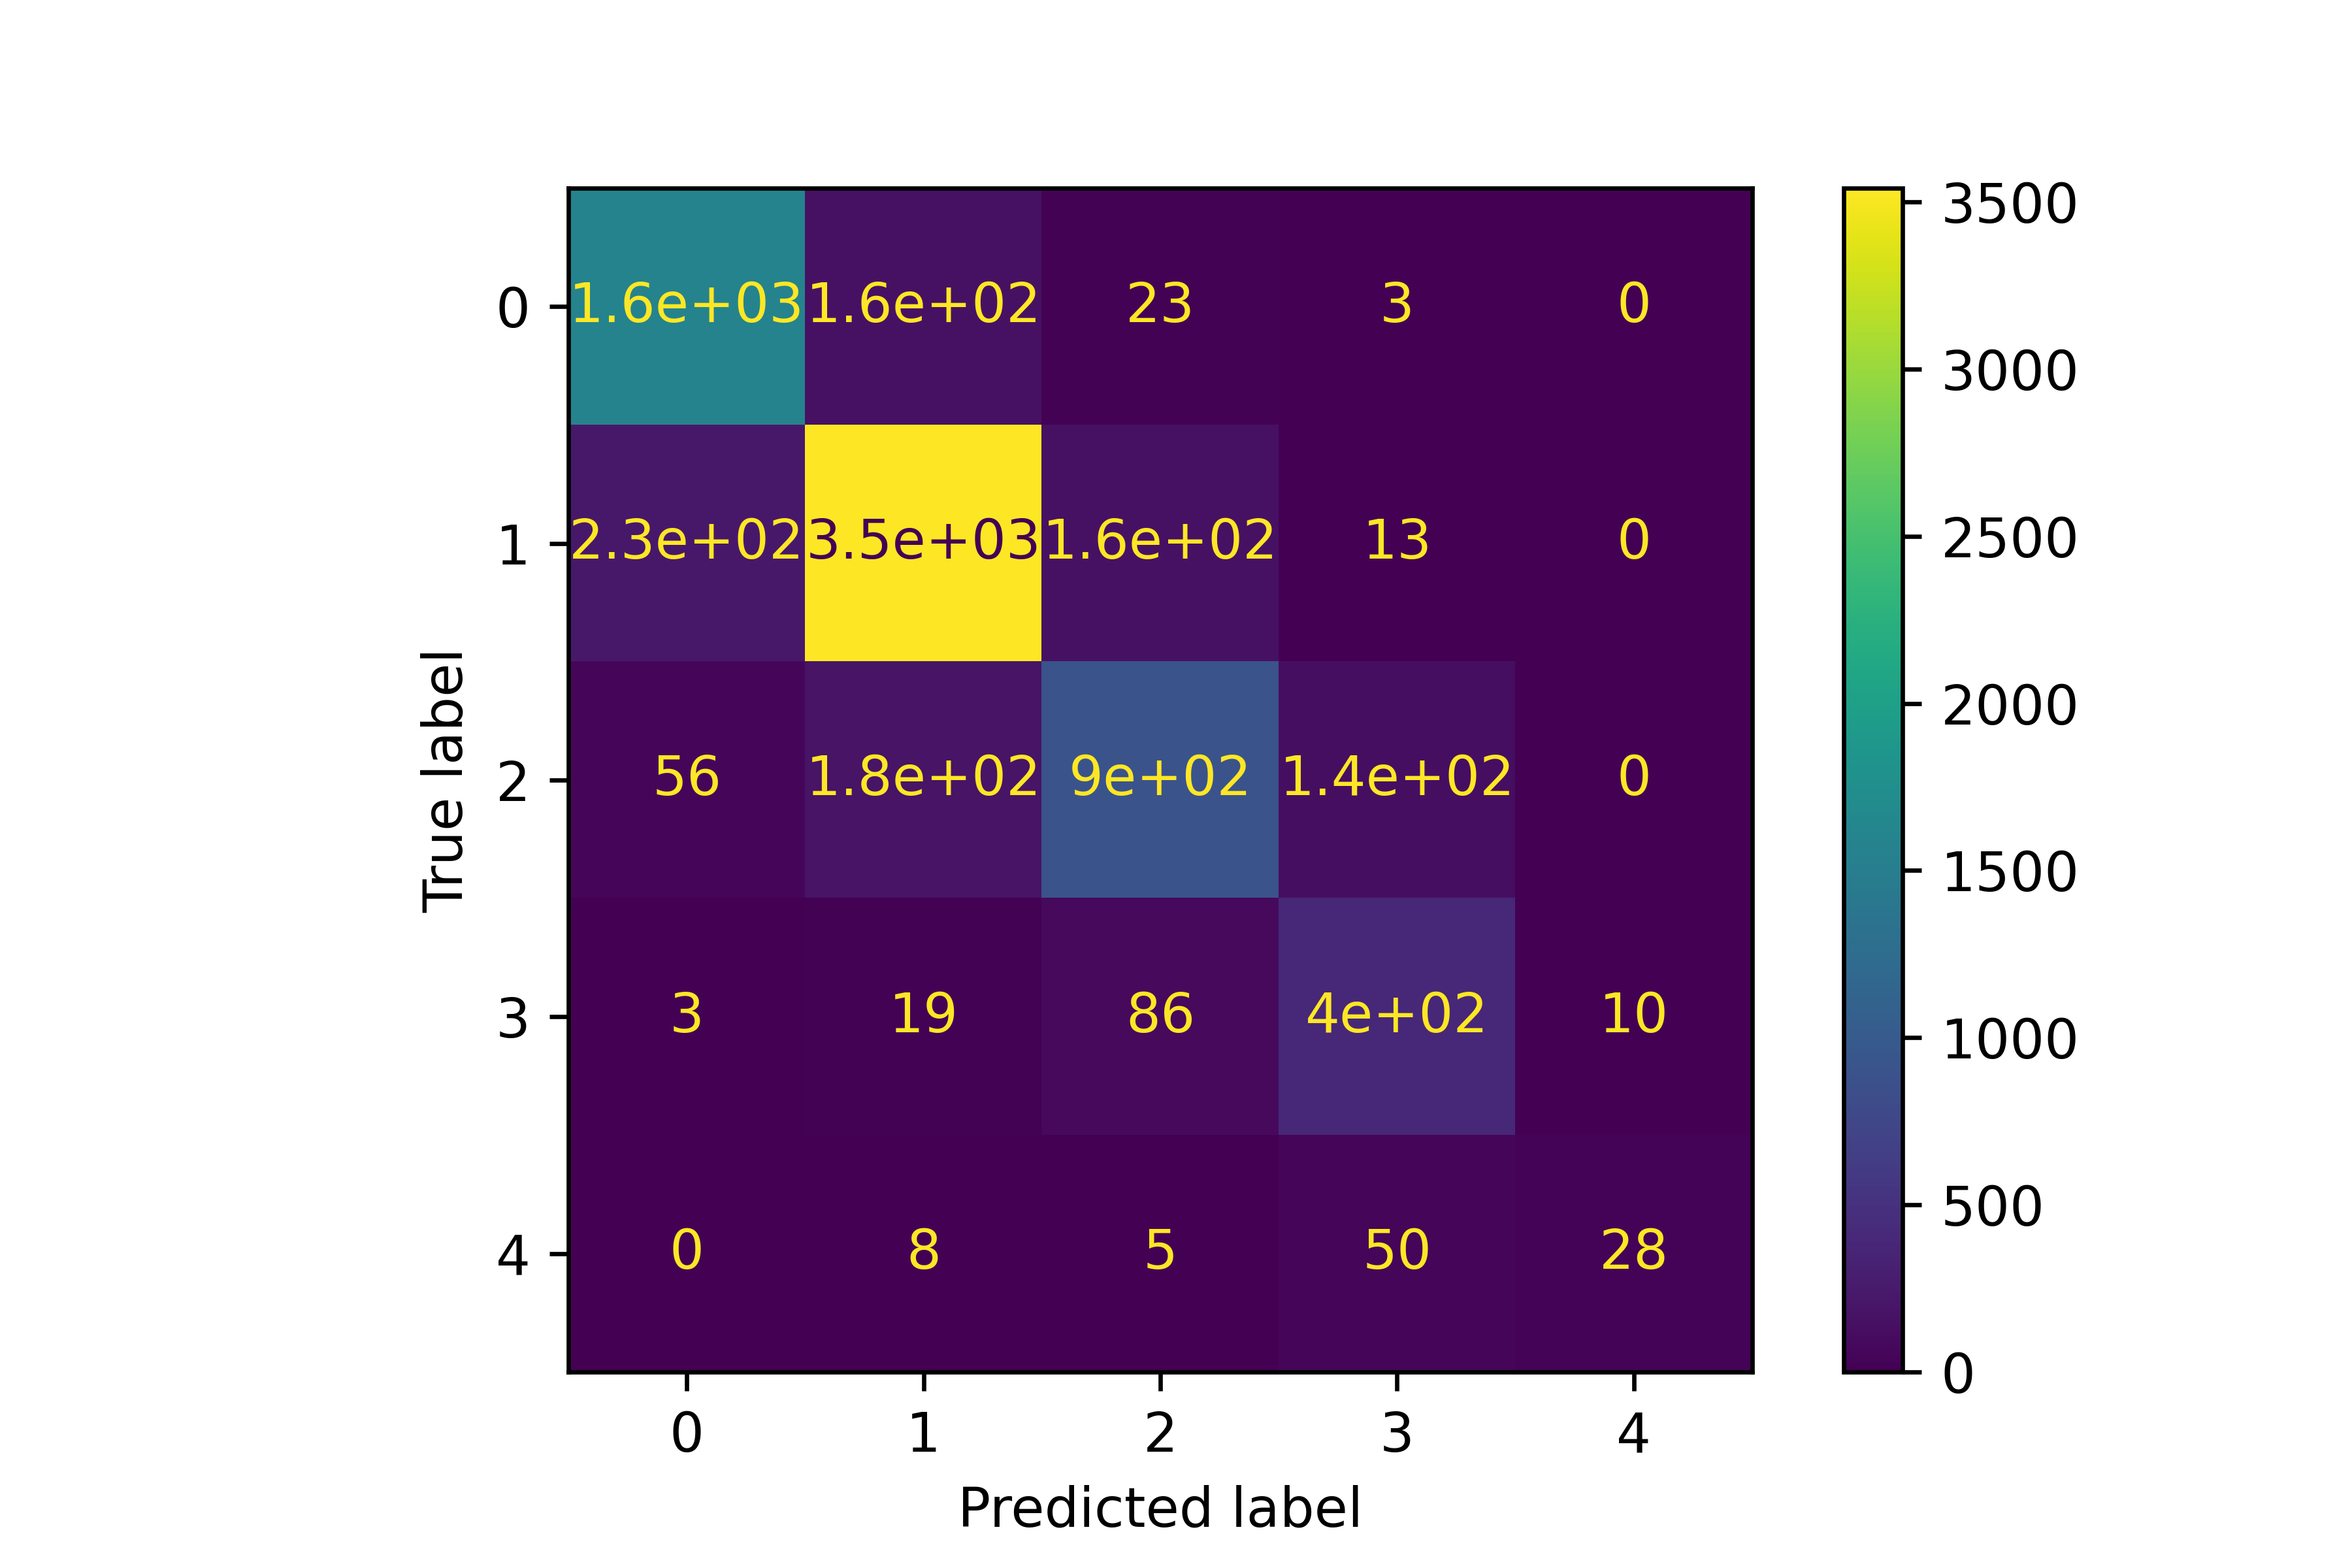
\includegraphics[width=\linewidth]{SVCConfusionMatrix.png}  
  \caption{}
%   \caption{Confusion Matrix for Support Vector Classifier}
  \label{subfig:svc}
\end{subfigure}


\caption{Confusion matrices for (a)Decision Tree, (b)Gradient Boost, (c)Random Forest, (d)Naive Bayes, (e)Bagging Classifier, (f)ANN, (g)SVC}
\label{fig:confusionMatrixForAllAlgos}
\end{figure}

\subsection{Results of model for suggesting plant based on a given water or soil sample}
\label{subsection:finalResults}
We apply the model given in Section 4.3 for suggesting plants based on a given water or soil sample. We suggest plants for 21,859 soil samples from lucas dataset\cite{dataset:lucas} and 37,999 water samples from major ions dataset\cite{dataset:majorIons}. Some soil and water samples didn't have suitable conditions so they were rejected. Plants were suggested for 13,700 soil samples and 29,114 water samples. 8,159 soil and 8,885 water samples were rejected. Results of 20 soil and water samples are given in Table \ref{table:soilPlantsResult} and Table \ref{table:waterPlantsResult} respectively.


\begin{table}[h!]
    \centering
    \begin{tabular}{|m{0.15\textwidth}|m{0.65\textwidth}|}
    \hline
        \textbf{Soil\_sample} & \textbf{List of plants suitable for the given soil sample} \\ \hline
        35163814 & 'Potatoes', 'Safflower', 'Fall rye', 'Oats', 'Yellow Mustard', 'Flax' \\ \hline
        34463934 & 'Safflower' \\ \hline
        33983238 & 'Safflower' \\ \hline
        34043240 & 'Potatoes', 'Safflower', 'Fall rye', 'Oats', 'Yellow Mustard', 'Flax' \\ \hline
        33723266 & 'Safflower' \\ \hline
        34123260 & 'Safflower', 'Fall rye', 'Oats' \\ \hline
        33523262 & 'Safflower' \\ \hline
        33683636 & 'Corn', 'Barley', 'Wheat ', 'Carrots', 'Strawberry', 'Tomato', 'Safflower', 'Fall rye', 'Oats', 'Yellow Mustard', 'Flax', 'Canola' \\ \hline
        34983634 & 'Safflower' \\ \hline
        33623332 & 'Garden Beet', 'Cabbage', 'Tomato', 'Broccoli', 'Asparagus', 'Spinach', 'Sunflower', 'Sugar beet', 'Safflower', 'Fall rye', 'Oats', 'Yellow Mustard', 'Flax' \\ \hline
        34383316 & 'Safflower', 'Fall rye', 'Oats', 'Yellow Mustard', 'Flax' \\ \hline
        34083328 & 'Safflower', 'Fall rye', 'Oats' \\ \hline
        34543252 & 'Garden Beet', 'Cabbage', 'Tomato', 'Broccoli', 'Asparagus', 'Spinach', 'Sunflower', 'Sugar beet', 'Safflower', 'Fall rye', 'Oats', 'Yellow Mustard', 'Flax' \\ \hline
        34883940 & 'Safflower' \\ \hline
        34683874 & 'Safflower', 'Fall rye', 'Oats' \\ \hline
        34823880 & 'Safflower', 'Fall rye', 'Oats' \\ \hline
        35623878 & 'Cabbage', 'Tomato', 'Broccoli', 'Asparagus', 'Spinach', 'Kochia', 'Sugar beet', 'Safflower', 'Fall rye', 'Oats', 'Yellow Mustard', 'Flax', 'Canola' \\ \hline
        36143890 & 'Corn', 'Barley', 'Wheat ', 'Tomato', 'Safflower', 'Fall rye', 'Oats', 'Yellow Mustard', 'Flax', 'Canola' \\ \hline
        35523886 & 'Safflower' \\ \hline
        35343868 & 'Safflower' \\ \hline
        34903806 & 'Safflower', 'Fall rye' \\ \hline
    \end{tabular}
    \caption{List of Plants for 20 soil samples out of 13,799 samples}
    \label{table:soilPlantsResult}
\end{table}

\begin{table}[H]
    \centering
    \begin{tabular}{|m{0.2\textwidth}|m{0.6\textwidth}|}
    \hline
        \textbf{Water\_sample} & \textbf{List of plants suitable for the given water sample} \\ \hline
        0 & 'Garden Beet', 'Potatoes', 'Corn', 'Barley', 'Wheat ', 'Cabbage', 'Tomato', 'Broccoli', 'Asparagus', 'Spinach', 'Sunflower', 'Kochia', 'Sugar beet', 'Safflower', 'Fall rye', 'Oats', 'Yellow Mustard', 'Flax', 'Canola' \\ \hline
        1 & 'Garden Beet', 'Barley', 'Wheat ', 'Cabbage', 'Tomato', 'Broccoli', 'Asparagus', 'Spinach', 'Sunflower', 'Kochia', 'Sugar beet', 'Safflower', 'Fall rye', 'Oats', 'Yellow Mustard', 'Flax', 'Canola' \\ \hline
        2 & 'Garden Beet', 'Barley', 'Wheat ', 'Asparagus', 'Spinach', 'Sunflower', 'Kochia', 'Sugar beet', 'Safflower', 'Fall rye' \\ \hline
        3 & 'Garden Beet', 'Barley', 'Wheat ', 'Cabbage', 'Tomato', 'Broccoli', 'Asparagus', 'Spinach', 'Sunflower', 'Kochia', 'Sugar beet', 'Safflower', 'Fall rye', 'Oats', 'Yellow Mustard', 'Flax', 'Canola' \\ \hline
        51 & 'Garden Beet', 'Barley', 'Wheat ', 'Cabbage', 'Tomato', 'Broccoli', 'Asparagus', 'Spinach', 'Sunflower', 'Kochia', 'Sugar beet', 'Safflower', 'Fall rye', 'Oats', 'Yellow Mustard', 'Flax', 'Canola' \\ \hline
        52 & 'Garden Beet', 'Potatoes', 'Corn', 'Barley', 'Wheat ', 'Cabbage', 'Tomato', 'Broccoli', 'Asparagus', 'Spinach', 'Sunflower', 'Kochia', 'Sugar beet', 'Safflower', 'Fall rye', 'Oats', 'Yellow Mustard', 'Flax', 'Canola' \\ \hline
        53 & 'Garden Beet', 'Barley', 'Wheat ', 'Cabbage', 'Tomato', 'Broccoli', 'Asparagus', 'Spinach', 'Sunflower', 'Kochia', 'Sugar beet', 'Safflower', 'Fall rye', 'Oats', 'Yellow Mustard', 'Flax', 'Canola' \\ \hline
        54 & 'Garden Beet', 'Barley', 'Wheat ', 'Cabbage', 'Tomato', 'Broccoli', 'Asparagus', 'Spinach', 'Sunflower', 'Kochia', 'Sugar beet', 'Safflower', 'Fall rye', 'Oats', 'Yellow Mustard', 'Flax', 'Canola' \\ \hline
        55 & 'Garden Beet', 'Potatoes', 'Corn', 'Barley', 'Wheat ', 'Cabbage', 'Tomato', 'Broccoli', 'Asparagus', 'Spinach', 'Sunflower', 'Kochia', 'Sugar beet', 'Safflower', 'Fall rye', 'Oats', 'Yellow Mustard', 'Flax', 'Canola' \\ \hline
        4 & 'Garden Beet', 'Barley', 'Wheat ', 'Asparagus', 'Spinach', 'Sunflower', 'Kochia', 'Sugar beet', 'Safflower', 'Fall rye' \\ \hline
        5 & 'Garden Beet', 'Barley', 'Wheat ', 'Asparagus', 'Spinach', 'Sunflower', 'Kochia', 'Sugar beet', 'Safflower', 'Fall rye' \\ \hline
        6 & 'Garden Beet', 'Barley', 'Wheat ', 'Asparagus', 'Spinach', 'Sunflower', 'Kochia', 'Sugar beet', 'Safflower', 'Fall rye' \\ \hline
        7 & 'Garden Beet', 'Barley', 'Wheat ', 'Asparagus', 'Spinach', 'Sunflower', 'Kochia', 'Sugar beet', 'Safflower', 'Fall rye' \\ \hline
        8 & 'Garden Beet', 'Barley', 'Wheat ', 'Asparagus', 'Spinach', 'Sunflower', 'Kochia', 'Sugar beet', 'Safflower', 'Fall rye' \\ \hline
        9 & 'Garden Beet', 'Potatoes', 'Corn', 'Barley', 'Wheat ', 'Cabbage', 'Tomato', 'Broccoli', 'Asparagus', 'Spinach', 'Sunflower', 'Kochia', 'Sugar beet', 'Safflower', 'Fall rye', 'Oats', 'Yellow Mustard', 'Flax', 'Canola' \\ \hline
        10 & 'Garden Beet', 'Potatoes', 'Corn', 'Barley', 'Wheat ', 'Cabbage', 'Tomato', 'Broccoli', 'Asparagus', 'Spinach', 'Sunflower', 'Kochia', 'Sugar beet', 'Safflower', 'Fall rye', 'Oats', 'Yellow Mustard', 'Flax', 'Canola' \\ \hline
        11 & 'Garden Beet', 'Barley', 'Wheat ', 'Asparagus', 'Spinach', 'Sunflower', 'Kochia', 'Sugar beet', 'Safflower', 'Fall rye' \\ \hline
        12 & 'Garden Beet', 'Barley', 'Wheat ', 'Asparagus', 'Spinach', 'Sunflower', 'Kochia', 'Sugar beet', 'Safflower', 'Fall rye' \\ \hline
        13 & 'Garden Beet', 'Barley', 'Wheat ', 'Asparagus', 'Spinach', 'Sunflower', 'Kochia', 'Sugar beet', 'Safflower', 'Fall rye' \\ \hline
        14 & 'Garden Beet', 'Barley', 'Wheat ', 'Asparagus', 'Spinach', 'Sunflower', 'Kochia', 'Sugar beet', 'Safflower', 'Fall rye' \\ \hline
    \end{tabular}
    \caption{List of Plants for 20 water samples out of 29,114 samples}
    \label{table:waterPlantsResult}
\end{table}

\section{Conclusion and Future Work}
\label{section:conclusionAndFutureWork}
We developed models for classifying water samples based on quality and suggesting plants based on soil and water parameters. We found out water samples  for quantifying water quality, we calculated Irrigation Water Quality Index(IWQI) of water samples using properties like Electrical Conductivity and Chemical Ion concentrations like Sodium, Chlorine etc of water. The index chosen is mainly focused on the effect of water on soil sodicity, salinity and toxicity. We assigned water quality classes to different ranges of IWQI values. Seven classification methods were used out of which Random Forest performed the best(86.9\%) followed by Gradient Boosting and Neural Networks on all of the evaluation methods used. For suggestions of plants based on water and soil properties, we converted the restrictions on soil salinity, pH and water quality for various plants to conditional statements. We were able to suggest plants for all the soil and water samples obtained except one third of soil and one fifth of water samples due to them being unfit for agricultural purposes.
Water quality taken in this work is mainly based on salinity of water samples whereas there can be many other parameters on which water quality can depend on like acidity, pollution level etc. Additionally, experiments can be done to see the effect of various water samples on plant growth keeping other factors like soil and weather as constant .The parameters mentioned can be used along with parameters used in our paper to develop an index covering more factors of water quality. The results can be further improved by collecting  more water samples from different types of water bodies. For soil samples, we only considered two parameters for suggestion of plants. More parameters like NPK, metals etc. can be measured along with plant growth data for the soil which can be used to develop a recommender system for recommending plants based on soil and water conditions.






 

%\begin{acknowledgements}
%If you'd like to thank anyone, place your comments here
%and remove the percent signs.
%\end{acknowledgements}


% Authors must disclose all relationships or interests that 
% could have direct or potential influence or impart bias on 
% the work: 
%
% \section*{Conflict of interest}
%
% The authors declare that they have no conflict of interest.


% BibTeX users please use one of
%\bibliographystyle{spbasic}      % basic style, author-year citations
%\bibliographystyle{spmpsci}      % mathematics and physical sciences
%\bibliographystyle{spphys}       % APS-like style for physics
%\bibliography{}   % name your BibTeX data base

% Non-BibTeX users please use
% \begin{thebibliography}{}
%
% and use \bibitem to create references. Consult the Instructions
% for authors for reference list style.
%
\bibliographystyle{IEEEtran}      
\bibliography{references} 


% etc

% \end{thebibliography}

\end{document}
% end of file template.tex

